% =============================================================================
% CAPÍTULO IV - RESULTADOS
% =============================================================================

\cleardoublepage
\thispagestyle{empty}
\vspace*{\fill}
\begin{center}
{\Large\bfseries CAPÍTULO IV}\\[2.5cm]
{\Large\bfseries RESULTADOS}
\end{center}
\vspace*{\fill}
\clearpage

\chapter*{}
\addcontentsline{toc}{chapter}{CAPÍTULO IV -- RESULTADOS}
\setcounter{chapter}{4}
\setcounter{section}{0}
\renewcommand{\thesection}{4.\arabic{section}}
\renewcommand{\thesubsection}{4.\arabic{section}.\arabic{subsection}}

\vspace{-3cm}

\section{Producto tecnológico desarrollado}

En esta sección se presentan los resultados obtenidos a lo largo del desarrollo del proyecto tecnológico Kiddy Quiz, habiendo alcanzado los objetivos planteados mediante la aplicación de la metodología ágil de Programación Extrema (XP). A través de iteraciones cortas, retroalimentación constante por parte de los docentes especialistas y la refactorización continua del código, se garantizó la entrega de un software alineado con las necesidades educativas. La presente sección detalla lo obtenido en cada etapa, comenzando por la obtención y análisis de los requisitos, continuando con el diseño y desarrollo del sistema, y finalizando con la fase de pruebas y validación, asegurando un producto de calidad, inclusivo y funcional para entornos reales. Adicionalmente, se presenta de manera detallada la comprobación de los indicadores de evaluación definidos en la sección 3.5. El manual de funcionamiento del sistema, dada su extensión y nivel de detalle visual, ha sido incluido en el Anexo~E.

De manera general, se obtuvo una aplicación web adaptativa totalmente funcional, estructurada en dos perfiles principales: estudiante y docente. El perfil del estudiante brinda un entorno accesible donde, al iniciar sesión, el usuario visualiza sus clases y puede unirse a nuevas mediante un código de acceso. Dentro de cada clase, el estudiante puede acceder a las evaluaciones asignadas, visualizar los detalles y resultados de sus pruebas, y consultar su progreso general. Una característica destacada es la integración de inteligencia artificial generativa (Gemini), la cual interviene brindando retroalimentación motivacional al finalizar cada prueba y generando contenido de refuerzo académico para fortalecer las competencias evaluadas. Por otro lado, el perfil del docente centraliza la gestión académica, mediante un módulo robusto que permite al profesor crear clases, gestionar estudiantes y administrar listas de evaluaciones, además de proveer analíticas y reportes detallados por estudiante.

\subsection{Obtención de requisitos}

Tras realizar las entrevistas y el trabajo de validación continua con los docentes especialistas, y una vez analizada toda la información recopilada (disponible en el Anexo~A), se definió el alcance del sistema. Esta información fue complementada con los lineamientos pedagógicos extraídos de la revisión bibliográfica para asegurar un enfoque adecuado hacia los estudiantes de educación básica.

Dado que el desarrollo se rigió bajo la metodología ágil de Programación Extrema (XP), la lista de requerimientos del sistema no se estructuró de forma tradicional, sino que se documentó directamente a través de veintinueve historias de usuario. En la Tabla~\ref{tab:hu} se muestra el listado consolidado de las historias de usuario que conforman el núcleo funcional de la aplicación.

\begin{table}[H]
\centering
\caption{Historias de usuario de la aplicación web Kiddy Quiz.}
\label{tab:hu}
\begin{footnotesize}
\begin{tabularx}{\textwidth}{|L{1.7cm}|L{3.5cm}|L{1.5cm}|X|X|}
\hline
\rowcolor{tabhead}
\tabhead{ID} & \tabhead{Título} & \tabhead{Como} & \tabhead{Quiero (acción)} & \tabhead{Para (beneficio)}\\
\hline
HU-001.1-F & Inicio de sesión y redirección & Usuario & Iniciar sesión con correo y contraseña & Acceder al panel correspondiente según perfil\\
\hline
HU-001.2-F & Cierre de sesión seguro & Usuario & Cerrar sesión activa mediante un botón & Proteger la información personal\\
\hline
HU-002.1-F & Registro unificado & Docente & Crear una cuenta eligiendo rol & Acceder sin necesidad de validación adicional\\
\hline
HU-002.2-F & Creación manual de alumnos & Docente & Crear cuentas directamente para mis alumnos & Facilitar el acceso y vinculación automática\\
\hline
HU-003.1-F & Panel de tarjetas (estudiante) & Estudiante & Ver evaluaciones asignadas en tarjetas visuales & Identificar rápidamente tema y dificultad\\
\hline
HU-004.1-F & Ejecución de evaluación & Estudiante & Responder preguntas de forma secuencial & Completar la prueba en un entorno amigable\\
\hline
HU-004.2-F & Soporte de control por voz & Estudiante & Activar funciones de voz en la evaluación & Interactuar de forma sencilla y autónoma\\
\hline
HU-005.1-F & \textit{Feedback} motivacional & Estudiante & Ver puntaje, tiempo y mensaje de ánimo & Sentirse motivado a mejorar\\
\hline
HU-006.1-F & Panel de gestión (docente) & Docente & Ver mis evaluaciones creadas en tarjetas & Gestionar contenido y visibilidad\\
\hline
HU-006.2-F & Habilitación rápida & Docente & Activar o desactivar pruebas con un interruptor & Controlar el acceso al examen\\
\hline
HU-006.3-F & Estructura base de evaluación & Docente & Definir tema, descripción, dificultad y duración & Establecer la configuración\\
\hline
HU-006.4-F & Modo lúdico & Estudiante & Realizar evaluaciones en formato de juego & Aprender divirtiéndose\\
\hline
HU-006.5-F & Programación temporal & Docente & Definir fechas de inicio y fin & Planificar el calendario académico\\
\hline
HU-006.6-F & Control de versiones & Docente & Mantener historial de modificaciones & Restaurar versiones en caso de errores\\
\hline
HU-006.7-F & Evaluaciones diagnósticas & Docente & Marcar pruebas como diagnósticas iniciales & Conocer el nivel previo del estudiante\\
\hline
HU-007.1-F & Gestión CRUD de preguntas & Docente & Editar, eliminar y reordenar preguntas & Estructurar el contenido pedagógico\\
\hline
HU-007.2-F & Creación de preguntas & Docente & Especificar enunciado, formato y respuestas & Calificar automáticamente\\
\hline
HU-007.3-F & Carga multimedia & Docente & Integrar imágenes, GIFs o videos & Brindar apoyo visual\\
\hline
HU-007.4-F & Preguntas interactivas & Docente & Configurar formatos como unir columnas o secuencias & Promover el pensamiento activo\\
\hline
HU-008.1-F & Lista de alumnos filtrable & Docente & Ver lista de alumnos por curso y buscador & Llevar un seguimiento del estado de los alumnos\\
\hline
HU-008.2-F & Panel de resultados detallados & Docente & Ver promedio global y desglose por evaluación & Evaluar el progreso individual\\
\hline
HU-008.3-F & Curva de mejora gráfica & Docente & Ver gráfica cronológica de puntajes & Identificar tendencias de aprendizaje\\
\hline
HU-008.4-F & Exportación a Excel & Docente & Descargar archivo .xlsx de rendimiento & Mantener respaldos administrativos\\
\hline
HU-008.5-F & Áreas fuertes y débiles & Docente & Ver análisis por categorías temáticas & Planificar refuerzos pedagógicos\\
\hline
HU-009.1-F & Sugerencias con IA & Usuario & Recibir sugerencias basadas en patrones de error & Saber qué temas reforzar\\
\hline
HU-010.1-F & Modo de lectura accesible & Estudiante & Que el sistema lea enunciados y opciones (TTS) & Ser autónomo en la lectura\\
\hline
HU-011.1-F & Ayudas contextuales & Estudiante & Acceder a pistas o definiciones & Comprender lenguaje abstracto\\
\hline
HU-012.1-F & Alertas de bajo rendimiento & Docente & Recibir notificaciones por notas bajas & Intervenir pedagógicamente a tiempo\\
\hline
HU-013.1-F & Mapa de competencias & Usuario & Ver mapa visual de competencias alcanzadas & Tener seguimiento del progreso académico\\
\hline
\end{tabularx}
\end{footnotesize}
\fuenteautor
\end{table}

En la Tabla~\ref{tab:rnf} se presenta el listado de requerimientos no funcionales obtenidos mediante revisión bibliográfica y entrevistas.

\begin{table}[H]
\centering
\caption{Requerimientos no funcionales de la aplicación web Kiddy Quiz.}
\label{tab:rnf}
\begin{small}
\begin{tabularx}{\textwidth}{|L{1.6cm}|L{4cm}|X|L{1.6cm}|}
\hline
\rowcolor{tabhead}
\tabhead{ID} & \tabhead{Nombre del requerimiento} & \tabhead{Descripción técnica} & \tabhead{Prioridad}\\
\hline
RNF-01 & Interfaz accesible e intuitiva & Uso de lenguaje simple, botones grandes y cumplimiento con la norma WCAG 2.1 nivel AA para inclusión & Alta\\
\hline
RNF-02 & Seguridad y protección de datos & Cifrado de contraseñas, protección contra ataques (XSS, SQL Injection) y cumplimiento de normativas de protección de datos & Crítica\\
\hline
RNF-03 & Rendimiento y concurrencia & Tiempo de respuesta inferior a 2 segundos y soporte para al menos 200 usuarios concurrentes & Media\\
\hline
RNF-04 & Mantenibilidad del sistema & Código modular, separación de lógica (NestJS) y presentación (Angular) con control de versiones Git & Media\\
\hline
RNF-05 & Escalabilidad del sistema & Arquitectura desacoplada preparada para añadir nodos y uso potencial de Docker/Kubernetes & Media\\
\hline
RNF-06 & Usabilidad para docentes & Panel con accesos rápidos y creación de evaluaciones mediante pasos guiados & Alta\\
\hline
\end{tabularx}
\end{small}
\fuenteautor
\end{table}

\subsection{Diagrama de casos de uso}

En la Ilustración~\ref{fig:casos_uso} se presenta el diagrama de casos de uso que contempla las funcionalidades centrales del sistema, representando el núcleo operativo de la aplicación web Kiddy Quiz (el diagrama completo se encuentra disponible en el Anexo~D). Este esquema refleja las interacciones principales entre la plataforma y los actores involucrados, los cuales corresponden al estudiante y al docente, quienes ejecutan acciones fundamentales para el desarrollo de la evaluación por competencias.

\begin{figure}[H]
\centering
\caption{Diagrama de casos de uso del sistema Kiddy Quiz.}
\label{fig:casos_uso}

\includegraphics[width=\textwidth]{figuras/fig03_casos_uso.pdf}
\fuenteautor
\end{figure}

El estudiante interactúa con la aplicación principalmente para visualizar las clases a las que pertenece, unirse a nuevas mediante un código de acceso y desarrollar las evaluaciones estructuradas por el docente. Adicionalmente, este perfil le permite consultar los detalles de sus resultados, monitorear su progreso académico general y acceder a la retroalimentación motivacional generada por la inteligencia artificial. Por su parte, las interacciones principales del docente consisten en la administración integral del entorno académico: el profesor utiliza el sistema para crear y gestionar clases, administrar el listado de estudiantes y emplear un editor completo para la creación de evaluaciones. Los casos de uso seleccionados se han elegido por su alta relevancia y alineación directa con los objetivos del proyecto.

\subsection{Descripción de los casos de uso extendidos}

A continuación se especifican los casos de uso derivados de la Ilustración~\ref{fig:casos_uso}. Para ello, se han seleccionado las interacciones más significativas del sistema, haciendo especial énfasis en las funcionalidades relacionadas con la evaluación por competencias. Cada caso de uso se documenta de manera consolidada en una tabla extendida que integra la descripción narrativa, el flujo de eventos escalonado entre actor y sistema, los flujos alternos, el diagrama de secuencia y la interfaz de usuario asociada.

% =============================================================================
% TABLA 12 - CASO DE USO "VER EVALUACIÓN"
% =============================================================================
\begin{small}
\begin{longtable}{|p{2.6cm}|p{4.0cm}|p{2.5cm}|p{3.8cm}|}
\caption{Caso de uso ``Ver evaluación''.}\label{tab:cu_ver_eval}\\
\hline
\rowcolor{tabhead}\multicolumn{4}{|c|}{\textbf{\textcolor{white}{Caso de uso ``Ver evaluación''}}}\\
\hline
\endfirsthead
\multicolumn{4}{c}{\tablename\ \thetable\ -- \textit{continuación}}\\
\hline
\rowcolor{tabhead}\multicolumn{4}{|c|}{\textbf{\textcolor{white}{Caso de uso ``Ver evaluación''}}}\\
\hline
\endhead
\textbf{Código:} & CU-003 & \textbf{Actores:} & Estudiante\\\hline
\cufield{Objetivo:}{Permitir que el estudiante visualice de forma organizada y atractiva las pruebas que su docente ha habilitado para su resolución.}
\cufield{Resumen:}{Al ingresar al sistema, el estudiante observa una cuadrícula de tarjetas que representan las evaluaciones activas, lo que le permite identificar temas y niveles de dificultad antes de comenzar.}
\cufield{Tipo:}{Principal.}
\cufield{Dependencias:}{\textbf{Invoca a:} CU-004 (Resolver evaluación). \textbf{Depende de:} Base de datos de evaluaciones, asociación estudiante-docente y filtros por estado.}
\cufield{Precondición:}{El estudiante debe estar autenticado y vinculado a un docente; debe existir al menos una evaluación en estado ``Habilitada''.}
\cufield{Postcondición:}{El estudiante visualiza las tarjetas interactivas en pantalla y el sistema queda a la espera de la selección de una prueba.}
\cufield{Importancia:}{Alta -- Es la interfaz principal de interacción y motivación para el estudiante.}
\cuhead{Flujo normal de eventos}
\rowcolor{tabhead2}\multicolumn{2}{|c|}{\textbf{Acción del actor}} & \multicolumn{2}{c|}{\textbf{Respuesta del sistema}}\\\hline
\cuactor{1.~El estudiante inicia sesión exitosamente en la plataforma (CU-001).}
\cusistema{2.~El sistema consulta las evaluaciones vinculadas al ID del docente y del estudiante.}
\cusistema{3.~El sistema filtra únicamente aquellas evaluaciones que tengan el estado ``Habilitada''.}
\cusistema{4.~La aplicación renderiza una cuadrícula de tarjetas con imagen, tema, descripción y dificultad.}
\cuactor{5.~El estudiante identifica y revisa la información de las tarjetas disponibles.}
\cuactor{6.~El estudiante selecciona una evaluación haciendo clic en la tarjeta deseada.}
\cusistema{7.~La aplicación redirige al estudiante a la pantalla de inicio de prueba (CU-004).}
\cuhead{Flujo alterno}
\multicolumn{4}{|p{13cm}|}{\textbf{3.a.~Sin evaluaciones disponibles:} si el docente no ha habilitado pruebas, el sistema muestra un mensaje amigable indicando que no hay tareas pendientes por el momento. \textbf{4.a.~Error de carga multimedia:} si las imágenes de las tarjetas no cargan, el sistema muestra un ícono temático por defecto para no interrumpir la navegación.}\\\hline
\cuhead{Diagrama de secuencia}
\cuimg{figuras/seq_ver_eval.pdf}
\cuhead{Interfaz de usuario}
\cuimg{figuras/ui_evaluaciones_estudiante.pdf}
\cufield{Comentarios:}{Las tarjetas deben cumplir con altos estándares de contraste y tamaño de fuente (WCAG 2.1) para asegurar la accesibilidad visual. En el \textit{frontend} con Angular se utiliza una tubería (\textit{pipe}) o filtro para organizar dinámicamente las tarjetas por fecha o dificultad.}
\multicolumn{4}{|r|}{\textit{\footnotesize Elaboración: Autor}}\\\hline
\end{longtable}
\end{small}

% =============================================================================
% TABLA 13 - CASO DE USO "RESOLVER EVALUACIÓN"
% =============================================================================
\begin{small}
\begin{longtable}{|p{2.6cm}|p{4.0cm}|p{2.5cm}|p{3.8cm}|}
\caption{Caso de uso ``Resolver evaluación''.}\label{tab:cu_resolver}\\
\hline
\rowcolor{tabhead}\multicolumn{4}{|c|}{\textbf{\textcolor{white}{Caso de uso ``Resolver evaluación''}}}\\
\hline
\endfirsthead
\multicolumn{4}{c}{\tablename\ \thetable\ -- \textit{continuación}}\\
\hline
\rowcolor{tabhead}\multicolumn{4}{|c|}{\textbf{\textcolor{white}{Caso de uso ``Resolver evaluación''}}}\\
\hline
\endhead
\textbf{Código:} & CU-004 & \textbf{Actores:} & Estudiante\\\hline
\cufield{Objetivo:}{Proporcionar un entorno interactivo y amigable para que el estudiante responda las preguntas de una evaluación de forma secuencial.}
\cufield{Resumen:}{El estudiante accede a la prueba, lee las instrucciones y responde los ítems uno a uno. El sistema permite navegación asistida, control por voz opcional y guarda el progreso automáticamente.}
\cufield{Tipo:}{Principal.}
\cufield{Dependencias:}{\textbf{Invoca a:} CU-005 (Ver retroalimentación). \textbf{Depende de:} motor de evaluación y base de datos de preguntas y respuestas.}
\cufield{Precondición:}{El estudiante debe haber seleccionado una evaluación válida y habilitada desde su panel de inicio (CU-003).}
\cufield{Postcondición:}{El sistema captura todas las respuestas y las envía al \textit{backend} para su cálculo y registro definitivo en la base de datos de desempeño.}
\cufield{Importancia:}{Muy alta -- Es el núcleo funcional para los estudiantes.}
\cuhead{Flujo normal de eventos}
\rowcolor{tabhead2}\multicolumn{2}{|c|}{\textbf{Acción del actor}} & \multicolumn{2}{c|}{\textbf{Respuesta del sistema}}\\\hline
\cuactor{1.~El estudiante selecciona una tarjeta de evaluación (CU-003).}
\cusistema{2.~La aplicación muestra una pantalla de ``Pre-evaluación'' con instrucciones claras.}
\cuactor{3.~El estudiante hace clic en el botón ``Comenzar''.}
\cusistema{4.~El sistema presenta la primera pregunta con sus respectivas opciones de respuesta.}
\cuactorsist{5.~(Opcional) El estudiante activa el control por voz para escuchar el enunciado.}{6.~El sistema sintetiza el texto y reproduce el audio del ítem actual.}
\cuactor{7.~El estudiante selecciona una respuesta y hace clic en el botón ``Siguiente''.}
\cusistema{8.~El sistema guarda la respuesta temporalmente y carga el siguiente ítem secuencialmente.}
\cuactor{9.~El estudiante repite los pasos 7 y 8 hasta completar todos los ítems.}
\cuactor{10.~Al finalizar la última pregunta, el estudiante hace clic en el botón ``Finalizar''.}
\cusistema{11.~El sistema procesa los datos y redirige a la pantalla de resultados (CU-005).}
\cuhead{Flujo alterno}
\multicolumn{4}{|p{13cm}|}{\textbf{4.a.~Evaluación con tiempo límite:} el sistema inicia un contador regresivo; si el tiempo se agota, se guarda lo avanzado y se finaliza la prueba automáticamente. \textbf{6.a.~Error de reproducción de voz:} si el navegador no soporta el audio, el sistema muestra una alerta sugiriendo continuar con la lectura visual. \textbf{8.a.~Desconexión de internet:} el sistema notifica la pérdida de conexión y mantiene las respuestas en caché local hasta que se restablezca el servicio.}\\\hline
\cuhead{Diagrama de secuencia}
\cuimg{figuras/seq_resolver_eval.pdf}
\cuhead{Interfaz de usuario}
\cuimg{figuras/ui_resolver_eval_pictograma.pdf}
\cufield{Comentarios:}{La interfaz debe ser totalmente responsiva y optimizada para dispositivos táctiles, facilitando la interacción de niños de primaria. El uso de \texttt{window.localStorage} en Angular asegura que el progreso no se pierda ante cierres accidentales.}
\multicolumn{4}{|r|}{\textit{\footnotesize Elaboración: Autor}}\\\hline
\end{longtable}
\end{small}

% =============================================================================
% TABLA 14 - CASO DE USO "VER RETROALIMENTACIÓN"
% =============================================================================
\begin{small}
\begin{longtable}{|p{2.6cm}|p{4.0cm}|p{2.5cm}|p{3.8cm}|}
\caption{Caso de uso ``Ver retroalimentación''.}\label{tab:cu_retro}\\
\hline
\rowcolor{tabhead}\multicolumn{4}{|c|}{\textbf{\textcolor{white}{Caso de uso ``Ver retroalimentación''}}}\\
\hline
\endfirsthead
\multicolumn{4}{c}{\tablename\ \thetable\ -- \textit{continuación}}\\
\hline
\rowcolor{tabhead}\multicolumn{4}{|c|}{\textbf{\textcolor{white}{Caso de uso ``Ver retroalimentación''}}}\\
\hline
\endhead
\textbf{Código:} & CU-005 & \textbf{Actores:} & Estudiante\\\hline
\cufield{Objetivo:}{Proporcionar al estudiante una visualización clara y motivadora de su desempeño académico inmediatamente después de completar una prueba.}
\cufield{Resumen:}{El sistema calcula la calificación, el tiempo empleado y genera una retroalimentación gráfica y motivacional para informar al estudiante sobre sus logros.}
\cufield{Tipo:}{Principal.}
\cufield{Dependencias:}{\textbf{Invoca a:} retorno a la pantalla principal (CU-003). \textbf{Depende de:} módulo de corrección automática, sistema gráfico de resultados y base de datos de desempeño.}
\cufield{Precondición:}{El estudiante debe haber finalizado y enviado satisfactoriamente las respuestas de su evaluación (CU-004). El \textit{backend} debe haber procesado y calculado la calificación final.}
\cufield{Postcondición:}{El estudiante visualiza su rendimiento y el estado de la evaluación cambia a ``Completada'' en la base de datos.}
\cufield{Importancia:}{Alta -- Aporta retroalimentación y cierre al proceso de aprendizaje.}
\cuhead{Flujo normal de eventos}
\rowcolor{tabhead2}\multicolumn{2}{|c|}{\textbf{Acción del actor}} & \multicolumn{2}{c|}{\textbf{Respuesta del sistema}}\\\hline
\cuactor{1.~El estudiante hace clic en el botón ``Finalizar'' de la evaluación (CU-004).}
\cusistema{2.~El sistema recibe las respuestas y ejecuta el algoritmo de calificación automática.}
\cusistema{3.~El sistema calcula el tiempo total empleado durante la sesión de prueba.}
\cusistema{4.~La aplicación renderiza una pantalla de resultados con el puntaje numérico obtenido.}
\cusistema{5.~El sistema genera y muestra un gráfico de desempeño con colores amigables.}
\cusistema{6.~El sistema muestra una imagen de \textit{feedback} motivacional basada en el rango de nota.}
\cuactorsist{7.~(Opcional) El estudiante selecciona ``Revisar respuestas'' si el docente habilitó la opción.}{8.~El sistema despliega el detalle de aciertos y errores cometidos.}
\cuactor{9.~El estudiante hace clic en ``Volver al inicio''.}
\cusistema{10.~La aplicación redirige al estudiante a su panel principal de evaluaciones (CU-003).}
\cuhead{Flujo alterno}
\multicolumn{4}{|p{13cm}|}{\textbf{2.a.~Error en el procesamiento:} si el cálculo de la nota falla, el sistema muestra un mensaje de error y guarda las respuestas para un reintento automático posterior. \textbf{8.a.~Revisión deshabilitada:} si el docente no permitió la revisión, el botón correspondiente no aparecerá en la interfaz de resultados.}\\\hline
\cuhead{Diagrama de secuencia}
\cuimg{figuras/seq_ver_retroalimentacion.pdf}
\cuhead{Interfaz de usuario}
\cuimg{figuras/ui_retroalimentacion.pdf}
\cufield{Comentarios:}{Los mensajes motivacionales deben estar adaptados a niños de primaria. Técnicamente, Angular recibe el objeto de resultados procesado por NestJS y utiliza librerías de gráficos para pintar la información de forma dinámica y responsiva.}
\multicolumn{4}{|r|}{\textit{\footnotesize Elaboración: Autor}}\\\hline
\end{longtable}
\end{small}

% =============================================================================
% TABLA 15 - CASO DE USO "GESTIONAR PANEL DOCENTE"
% =============================================================================
\begin{small}
\begin{longtable}{|p{2.6cm}|p{4.0cm}|p{2.5cm}|p{3.8cm}|}
\caption{Caso de uso ``Gestionar panel docente''.}\label{tab:cu_panel}\\
\hline
\rowcolor{tabhead}\multicolumn{4}{|c|}{\textbf{\textcolor{white}{Caso de uso ``Gestionar panel docente''}}}\\
\hline
\endfirsthead
\multicolumn{4}{c}{\tablename\ \thetable\ -- \textit{continuación}}\\
\hline
\rowcolor{tabhead}\multicolumn{4}{|c|}{\textbf{\textcolor{white}{Caso de uso ``Gestionar panel docente''}}}\\
\hline
\endhead
\textbf{Código:} & CU-006 & \textbf{Actores:} & Docente\\\hline
\cufield{Objetivo:}{Visualizar todas las evaluaciones que el docente ha creado, organizadas en formato de tarjetas informativas desde su pantalla principal.}
\cufield{Resumen:}{El docente accede a su panel principal donde el sistema filtra y muestra exclusivamente sus evaluaciones, permitiéndole conocer el estado de visibilidad y acceder a su edición.}
\cufield{Tipo:}{Principal.}
\cufield{Dependencias:}{\textbf{Invoca a:} CU-008 (Crear examen) y CU-007 (Habilitación y deshabilitación). \textbf{Depende de:} base de datos de evaluaciones y autenticación.}
\cufield{Precondición:}{El docente debe haber iniciado sesión y tener un \textit{token} de autenticación válido.}
\cufield{Postcondición:}{El sistema despliega la lista de tarjetas de las pruebas creadas por el docente, habilitando el acceso rápido a la edición de cada una.}
\cufield{Importancia:}{Alta -- Facilita la gestión directa del contenido por parte del docente.}
\cuhead{Flujo normal de eventos}
\rowcolor{tabhead2}\multicolumn{2}{|c|}{\textbf{Acción del actor}} & \multicolumn{2}{c|}{\textbf{Respuesta del sistema}}\\\hline
\cuactor{1.~El docente inicia sesión exitosamente en la plataforma (CU-001).}
\cusistema{2.~El sistema identifica el ID del docente autenticado en la base de datos.}
\cusistema{3.~El sistema filtra exclusivamente las evaluaciones asociadas a dicho ID.}
\cusistema{4.~La aplicación renderiza en el panel principal una cuadrícula con tarjetas informativas.}
\cuactor{5.~El docente revisa el nombre, descripción, dificultad y estado de sus pruebas.}
\cuactor{6.~El docente selecciona el ícono de ``acceso rápido'' en una tarjeta específica.}
\cusistema{7.~La aplicación redirige al docente a la interfaz de edición de esa evaluación.}
\cuhead{Flujo alterno}
\multicolumn{4}{|p{13cm}|}{\textbf{3.a.~Docente sin evaluaciones:} si no ha creado contenido, el sistema muestra un mensaje y ofrece un botón destacado para ``Crear nueva evaluación''. \textbf{4.a.~Error de carga:} si el servidor no responde, la interfaz muestra una alerta y permite reintentar.}\\\hline
\cuhead{Diagrama de secuencia}
\cuimg{figuras/seq_panel_docente.pdf}
\cuhead{Interfaz de usuario}
\cuimg{figuras/ui_panel_docente_clases.pdf}
\cufield{Comentarios:}{El diseño debe ser totalmente responsivo, garantizando la gestión desde computadoras o dispositivos móviles. En PostgreSQL se utiliza el ID del docente como llave foránea para asegurar el aislamiento de datos entre profesores.}
\multicolumn{4}{|r|}{\textit{\footnotesize Elaboración: Autor}}\\\hline
\end{longtable}
\end{small}

% =============================================================================
% TABLA 16 - CASO DE USO "CREAR EXAMEN"
% =============================================================================
\begin{small}
\begin{longtable}{|p{2.6cm}|p{4.0cm}|p{2.5cm}|p{3.8cm}|}
\caption{Caso de uso ``Crear examen''.}\label{tab:cu_crear_examen}\\
\hline
\rowcolor{tabhead}\multicolumn{4}{|c|}{\textbf{\textcolor{white}{Caso de uso ``Crear examen''}}}\\
\hline
\endfirsthead
\multicolumn{4}{c}{\tablename\ \thetable\ -- \textit{continuación}}\\
\hline
\rowcolor{tabhead}\multicolumn{4}{|c|}{\textbf{\textcolor{white}{Caso de uso ``Crear examen''}}}\\
\hline
\endhead
\textbf{Código:} & CU-008 & \textbf{Actores:} & Docente\\\hline
\cufield{Objetivo:}{Permitir al docente definir la estructura base de una nueva evaluación (tema, dificultad, descripción y duración) antes de agregar las preguntas.}
\cufield{Resumen:}{El docente ingresa los datos generales de la prueba en un formulario; el sistema valida la información y crea el registro en la base de datos en estado borrador.}
\cufield{Tipo:}{Principal.}
\cufield{Dependencias:}{\textbf{Invoca a:} CU-009 (Organizar preguntas). \textbf{Depende de:} interfaz de gestión docente y base de datos de evaluaciones.}
\cufield{Precondición:}{El docente debe haber iniciado sesión, contar con los permisos adecuados y encontrarse en su panel de gestión.}
\cufield{Postcondición:}{La nueva evaluación queda registrada en la base de datos vinculada al docente, habilitando la interfaz para agregar preguntas.}
\cufield{Importancia:}{Muy alta -- Es la funcionalidad base del sistema de evaluación.}
\cuhead{Flujo normal de eventos}
\rowcolor{tabhead2}\multicolumn{2}{|c|}{\textbf{Acción del actor}} & \multicolumn{2}{c|}{\textbf{Respuesta del sistema}}\\\hline
\cuactor{1.~El docente selecciona la opción ``Crear nueva evaluación''.}
\cusistema{2.~El sistema muestra el formulario vacío de creación de evaluación.}
\cuactor{3.~El docente completa los campos obligatorios: título, dificultad, descripción y duración.}
\cuactor{4.~El docente hace clic en el botón ``Crear evaluación''.}
\cusistema{5.~El sistema valida que los campos requeridos no estén vacíos y la duración sea positiva.}
\cusistema{6.~El sistema registra la nueva evaluación en la base de datos PostgreSQL.}
\cusistema{7.~La aplicación redirige al docente a la interfaz de gestión de preguntas (CU-009).}
\cuhead{Flujos alternos}
\multicolumn{4}{|p{13cm}|}{\textbf{5.a.}~Si el docente deja campos obligatorios vacíos, el sistema resalta los errores en rojo y detiene el guardado. \textbf{5.b.}~Si se ingresa una duración negativa o cero, el sistema solicita un número válido antes de continuar.}\\\hline
\cuhead{Diagrama de secuencia}
\cuimg{figuras/seq_crear_examen.pdf}
\cuhead{Interfaz de usuario}
\cuimg{figuras/ui_crear_examen.pdf}
\cufield{Comentarios:}{Se recomienda agregar asistencia visual en la interfaz (textos de ejemplo o plantillas prediseñadas) para facilitar la carga de datos al docente.}
\multicolumn{4}{|r|}{\textit{\footnotesize Elaboración: Autor}}\\\hline
\end{longtable}
\end{small}

% =============================================================================
% TABLA 17 - CASO DE USO "ORGANIZAR PREGUNTAS"
% =============================================================================
\begin{small}
\begin{longtable}{|p{2.6cm}|p{4.0cm}|p{2.5cm}|p{3.8cm}|}
\caption{Caso de uso ``Organizar preguntas''.}\label{tab:cu_org_preg}\\
\hline
\rowcolor{tabhead}\multicolumn{4}{|c|}{\textbf{\textcolor{white}{Caso de uso ``Organizar preguntas''}}}\\
\hline
\endfirsthead
\multicolumn{4}{c}{\tablename\ \thetable\ -- \textit{continuación}}\\
\hline
\rowcolor{tabhead}\multicolumn{4}{|c|}{\textbf{\textcolor{white}{Caso de uso ``Organizar preguntas''}}}\\
\hline
\endhead
\textbf{Código:} & CU-009 & \textbf{Actores:} & Docente\\\hline
\cufield{Objetivo:}{Permitir al docente gestionar la lista de preguntas asociadas a una evaluación específica mediante visualización, edición, eliminación y reordenamiento.}
\cufield{Resumen:}{El docente accede al administrador de una prueba para ver y modificar las preguntas existentes. El sistema procesa las acciones CRUD y actualiza la estructura en la base de datos.}
\cufield{Tipo:}{Principal.}
\cufield{Dependencias:}{\textbf{Invoca a:} CU-010 (Configurar contenido). \textbf{Depende de:} evaluación previamente creada (CU-008) y base de datos de preguntas.}
\cufield{Precondición:}{El docente debe haber iniciado sesión y haber creado previamente al menos una evaluación.}
\cufield{Postcondición:}{El sistema actualiza la estructura de la evaluación reflejando cualquier modificación, eliminación o cambio de orden.}
\cufield{Importancia:}{Muy alta -- Fundamental para personalizar y estructurar las evaluaciones.}
\cuhead{Flujo normal de eventos}
\rowcolor{tabhead2}\multicolumn{2}{|c|}{\textbf{Acción del actor}} & \multicolumn{2}{c|}{\textbf{Respuesta del sistema}}\\\hline
\cuactor{1.~El docente selecciona una evaluación y da clic en ``Gestionar preguntas''.}
\cusistema{2.~El sistema consulta y muestra la lista editable con todas las preguntas asociadas.}
\cuactor{3.~El docente cambia el orden de las preguntas (\textit{drag \& drop}).}
\cusistema{4.~El sistema actualiza visualmente el orden de la lista en la pantalla.}
\cuactor{5.~El docente da clic en el botón ``Guardar'' o ``Confirmar cambios''.}
\cusistema{6.~El sistema registra el nuevo orden en la base de datos y muestra un mensaje de éxito.}
\cuhead{Flujos alternos}
\multicolumn{4}{|p{13cm}|}{\textbf{2.a.}~Si la evaluación aún no tiene preguntas, el sistema muestra un mensaje y destaca el botón para crear una nueva (CU-010). \textbf{3.a.}~Si en lugar de ordenar, el docente elige ``Eliminar'' una pregunta, el sistema despliega un modal de confirmación obligatoria. Si el docente cancela, la acción se aborta.}\\\hline
\cuhead{Diagrama de secuencia}
\cuimg{figuras/seq_organizar_preguntas.pdf}
\cuhead{Interfaz de usuario}
\cuimg{figuras/ui_nueva_pregunta.pdf}
\cufield{Comentarios:}{Se sugiere incluir botones de navegación amigables para moverse entre la lista de preguntas y la configuración general. Se beneficia directamente de un control de versiones (CU-023).}
\multicolumn{4}{|r|}{\textit{\footnotesize Elaboración: Autor}}\\\hline
\end{longtable}
\end{small}

% =============================================================================
% TABLA 18 - CASO DE USO "CONFIGURAR CONTENIDO"
% =============================================================================
\begin{small}
\begin{longtable}{|p{2.6cm}|p{4.0cm}|p{2.5cm}|p{3.8cm}|}
\caption{Caso de uso ``Configurar contenido''.}\label{tab:cu_config}\\
\hline
\rowcolor{tabhead}\multicolumn{4}{|c|}{\textbf{\textcolor{white}{Caso de uso ``Configurar contenido''}}}\\
\hline
\endfirsthead
\multicolumn{4}{c}{\tablename\ \thetable\ -- \textit{continuación}}\\
\hline
\rowcolor{tabhead}\multicolumn{4}{|c|}{\textbf{\textcolor{white}{Caso de uso ``Configurar contenido''}}}\\
\hline
\endhead
\textbf{Código:} & CU-010 & \textbf{Actores:} & Docente\\\hline
\cufield{Objetivo:}{Permitir al docente crear preguntas estructuradas para una evaluación, definiendo el enunciado, el formato y las opciones de respuesta válidas.}
\cufield{Resumen:}{El docente selecciona el tipo de pregunta, redacta el enunciado y configura las opciones indicando cuál es la correcta. El sistema valida la integridad de la pregunta y la guarda.}
\cufield{Tipo:}{Principal.}
\cufield{Dependencias:}{\textbf{Invoca a:} CU-011 (Adjuntar archivos multimedia). \textbf{Depende de:} evaluación existente e interfaz de edición docente.}
\cufield{Precondición:}{El docente debe estar autenticado, haber seleccionado una evaluación y encontrarse dentro de la interfaz de gestión de preguntas (CU-009).}
\cufield{Postcondición:}{La nueva pregunta, junto con su enunciado, tipo y estructura de respuestas, se registra en la base de datos asociada al ID de la evaluación.}
\cufield{Importancia:}{Muy alta -- Permite generar contenido pedagógico evaluativo y la calificación automática.}
\cuhead{Flujo normal de eventos}
\rowcolor{tabhead2}\multicolumn{2}{|c|}{\textbf{Acción del actor}} & \multicolumn{2}{c|}{\textbf{Respuesta del sistema}}\\\hline
\cuactor{1.~El docente da clic en la opción para agregar un nuevo ítem evaluativo.}
\cusistema{2.~El sistema provee un formulario con un campo de texto enriquecido y un selector de tipo de pregunta.}
\cuactor{3.~El docente ingresa el enunciado y selecciona el formato (múltiple, V/F o corta).}
\cusistema{4.~El sistema adapta dinámicamente los campos para ingresar las opciones de respuesta.}
\cuactor{5.~El docente llena las opciones y marca explícitamente cuál es la correcta.}
\cuactor{6.~El docente hace clic en ``Guardar''.}
\cusistema{7.~El sistema verifica la información y registra la pregunta en la base de datos.}
\cusistema{8.~La aplicación actualiza la vista mostrando la nueva pregunta en la lista.}
\cuhead{Flujos alternos}
\multicolumn{4}{|p{13cm}|}{\textbf{7.a.}~Si el docente olvida marcar al menos una respuesta como correcta, el sistema aplica una validación que impide guardar y resalta el error. \textbf{5.a.}~Antes de guardar, el docente puede usar ``Vista previa'' y el sistema renderizará la pregunta tal como la verá el estudiante.}\\\hline
\cuhead{Diagrama de secuencia}
\cuimg{figuras/seq_configurar_contenido.pdf}
\cuhead{Interfaz de usuario}
\cuimg{figuras/ui_gestionar_opciones.pdf}
\cufield{Comentarios:}{La validación de la respuesta correcta es crítica para que el motor de evaluación (CU-004) pueda funcionar. El campo de enunciado debe soportar texto enriquecido.}
\multicolumn{4}{|r|}{\textit{\footnotesize Elaboración: Autor}}\\\hline
\end{longtable}
\end{small}

% =============================================================================
% TABLA 19 - CASO DE USO "ADJUNTAR ARCHIVOS MULTIMEDIA"
% =============================================================================
\begin{small}
\begin{longtable}{|p{2.6cm}|p{4.0cm}|p{2.5cm}|p{3.8cm}|}
\caption{Caso de uso ``Adjuntar archivos multimedia''.}\label{tab:cu_multimedia}\\
\hline
\rowcolor{tabhead}\multicolumn{4}{|c|}{\textbf{\textcolor{white}{Caso de uso ``Adjuntar archivos multimedia''}}}\\
\hline
\endfirsthead
\multicolumn{4}{c}{\tablename\ \thetable\ -- \textit{continuación}}\\
\hline
\rowcolor{tabhead}\multicolumn{4}{|c|}{\textbf{\textcolor{white}{Caso de uso ``Adjuntar archivos multimedia''}}}\\
\hline
\endhead
\textbf{Código:} & CU-011 & \textbf{Actores:} & Docente\\\hline
\cufield{Objetivo:}{Permitir al docente cargar e integrar recursos multimedia (imágenes, GIFs o videos) en las preguntas para enriquecer visualmente la evaluación.}
\cufield{Resumen:}{El docente sube un archivo multimedia al editor de preguntas. El sistema valida la extensión y el tamaño, muestra una vista previa y vincula la URL del archivo a la pregunta.}
\cufield{Tipo:}{Secundario (extensión de CU-010).}
\cufield{Dependencias:}{\textbf{Invoca a:} ninguno directamente, es extensión de CU-010. \textbf{Depende de:} módulo de creación de preguntas y sistema de almacenamiento de archivos.}
\cufield{Precondición:}{El docente debe estar autenticado y encontrarse dentro de la interfaz de creación o edición de una pregunta específica (CU-010).}
\cufield{Postcondición:}{El archivo multimedia se procesa, se guarda y su URL se vincula a la pregunta correspondiente respetando la posición configurada.}
\cufield{Importancia:}{Alta -- Aumenta la comprensión en alumnos con diferentes estilos de aprendizaje.}
\cuhead{Flujo normal de eventos}
\rowcolor{tabhead2}\multicolumn{2}{|c|}{\textbf{Acción del actor}} & \multicolumn{2}{c|}{\textbf{Respuesta del sistema}}\\\hline
\cuactor{1.~El docente interactúa con la zona de carga de archivos (\textit{drag \& drop} o botón) en el editor.}
\cusistema{2.~El sistema habilita la selección o recepción del recurso multimedia.}
\cuactor{3.~El docente selecciona un archivo e indica la posición (arriba o abajo del enunciado).}
\cusistema{4.~El sistema valida que la extensión sea .jpg, .png, .gif o .mp4 y no exceda el tamaño.}
\cusistema{5.~Al cargar el archivo con éxito, la interfaz genera y muestra una vista previa en tiempo real.}
\cuactor{6.~El docente finaliza y guarda la pregunta.}
\cusistema{7.~El sistema almacena el recurso y vincula su URL a la pregunta en la base de datos.}
\cuhead{Flujos alternos}
\multicolumn{4}{|p{13cm}|}{\textbf{4.a.~Formato no soportado:} si el archivo no tiene extensión válida, el sistema rechaza la carga y muestra un error. \textbf{4.b.~Exceso de tamaño:} si supera el límite permitido, el sistema advierte y detiene la carga.}\\\hline
\cuhead{Diagrama de secuencia}
\cuimg{figuras/seq_adjuntar_multimedia.pdf}
\cuhead{Interfaz de usuario}
\cuimg{figuras/ui_arasaac_pictogramas.pdf}
\cufield{Comentarios:}{Se debe verificar la compatibilidad con dispositivos móviles y limitar el tamaño de los archivos para asegurar buen rendimiento. Los recursos deben renderizarse responsivamente.}
\multicolumn{4}{|r|}{\textit{\footnotesize Elaboración: Autor}}\\\hline
\end{longtable}
\end{small}

% =============================================================================
% TABLA 20 - CASO DE USO "CONSULTAR ALUMNOS"
% =============================================================================
\begin{small}
\begin{longtable}{|p{2.6cm}|p{4.0cm}|p{2.5cm}|p{3.8cm}|}
\caption{Caso de uso ``Consultar alumnos''.}\label{tab:cu_alumnos}\\
\hline
\rowcolor{tabhead}\multicolumn{4}{|c|}{\textbf{\textcolor{white}{Caso de uso ``Consultar alumnos''}}}\\
\hline
\endfirsthead
\multicolumn{4}{c}{\tablename\ \thetable\ -- \textit{continuación}}\\
\hline
\rowcolor{tabhead}\multicolumn{4}{|c|}{\textbf{\textcolor{white}{Caso de uso ``Consultar alumnos''}}}\\
\hline
\endhead
\textbf{Código:} & CU-012 & \textbf{Actores:} & Docente\\\hline
\cufield{Objetivo:}{Visualizar una lista completa y filtrable de los alumnos vinculados al docente, organizados por curso o grupo, para llevar un seguimiento de su estado.}
\cufield{Resumen:}{El docente accede a la sección de estudiantes y el sistema despliega una tabla con los alumnos del docente. Permite filtrar por nombre mediante un buscador.}
\cufield{Tipo:}{Principal.}
\cufield{Dependencias:}{\textbf{Invoca a:} CU-013 (Analizar calificaciones). \textbf{Depende de:} módulo de registro, asociación alumno-docente y base de datos de usuarios.}
\cufield{Precondición:}{El docente debe haber iniciado sesión y debe existir al menos un estudiante vinculado al código único del docente (CU-002).}
\cufield{Postcondición:}{El sistema despliega correctamente la lista de alumnos según los filtros aplicados.}
\cufield{Importancia:}{Alta -- Permite acceder rápidamente al seguimiento individual.}
\cuhead{Flujo normal de eventos}
\rowcolor{tabhead2}\multicolumn{2}{|c|}{\textbf{Acción del actor}} & \multicolumn{2}{c|}{\textbf{Respuesta del sistema}}\\\hline
\cuactor{1.~El docente accede a la sección de gestión de estudiantes.}
\cusistema{2.~El sistema identifica el ID del docente y consulta los alumnos vinculados.}
\cusistema{3.~La aplicación muestra una lista organizada por curso, indicando: nombre, curso/grupo y estado.}
\cusistema{4.~El sistema muestra un contador del total de alumnos inscritos por cada grupo.}
\cuactor{5.~El docente utiliza el buscador ingresando el nombre de un alumno específico.}
\cusistema{6.~El sistema filtra los resultados en tiempo real mostrando coincidencias parciales o exactas.}
\cuactor{7.~El docente selecciona a un estudiante de la lista.}
\cusistema{8.~El sistema redirige a la vista de perfil de rendimiento del estudiante (CU-013).}
\cuhead{Flujos alternos}
\multicolumn{4}{|p{13cm}|}{\textbf{3.a.}~Si el docente no tiene alumnos vinculados, el sistema muestra un mensaje y le recuerda su código de vinculación. \textbf{6.a.}~Si la búsqueda no arroja coincidencias, el sistema muestra ``No se encontraron alumnos'' y permite limpiar el buscador.}\\\hline
\cuhead{Diagrama de secuencia}
\cuimg{figuras/seq_consultar_alumnos.pdf}
\cuhead{Interfaz de usuario}
\cuimg{figuras/ui_listado_estudiantes.pdf}
\cufield{Comentarios:}{La interfaz debe ser limpia y responsiva, garantizando que la tabla se adapte correctamente a pantallas de dispositivos móviles sin perder columnas.}
\multicolumn{4}{|r|}{\textit{\footnotesize Elaboración: Autor}}\\\hline
\end{longtable}
\end{small}

% =============================================================================
% TABLA 21 - CASO DE USO "ANALIZAR CALIFICACIONES"
% =============================================================================
\begin{small}
\begin{longtable}{|p{2.6cm}|p{4.0cm}|p{2.5cm}|p{3.8cm}|}
\caption{Caso de uso ``Analizar calificaciones''.}\label{tab:cu_analizar}\\
\hline
\rowcolor{tabhead}\multicolumn{4}{|c|}{\textbf{\textcolor{white}{Caso de uso ``Analizar calificaciones''}}}\\
\hline
\endfirsthead
\multicolumn{4}{c}{\tablename\ \thetable\ -- \textit{continuación}}\\
\hline
\rowcolor{tabhead}\multicolumn{4}{|c|}{\textbf{\textcolor{white}{Caso de uso ``Analizar calificaciones''}}}\\
\hline
\endhead
\textbf{Código:} & CU-013 & \textbf{Actores:} & Docente\\\hline
\cufield{Objetivo:}{Acceder al perfil académico de un estudiante para visualizar su promedio global y el desglose de resultados por cada evaluación realizada.}
\cufield{Resumen:}{El docente selecciona a un estudiante para evaluar su progreso. El sistema calcula y muestra el promedio acumulado junto con el detalle de cada prueba.}
\cufield{Tipo:}{Principal.}
\cufield{Dependencias:}{\textbf{Invoca a:} CU-014 (Curva de mejora) y CU-015 (Exportación). \textbf{Depende de:} evaluaciones realizadas y motor de análisis (CU-012).}
\cufield{Precondición:}{El docente debe estar autenticado, encontrarse en la lista de alumnos (CU-012) y seleccionar a un estudiante con al menos una evaluación completada.}
\cufield{Postcondición:}{El sistema presenta el promedio general del estudiante y los resultados desglosados (puntaje, fecha, duración).}
\cufield{Importancia:}{Muy alta -- Fundamental para evaluar el progreso del alumno.}
\cuhead{Flujo normal de eventos}
\rowcolor{tabhead2}\multicolumn{2}{|c|}{\textbf{Acción del actor}} & \multicolumn{2}{c|}{\textbf{Respuesta del sistema}}\\\hline
\cuactor{1.~El docente hace clic en un alumno desde la ``Lista de alumnos'' (CU-012).}
\cusistema{2.~El sistema consulta el historial de evaluaciones completadas por el estudiante.}
\cusistema{3.~El sistema calcula el promedio general acumulado del estudiante.}
\cusistema{4.~La aplicación muestra el perfil destacando visualmente el promedio global.}
\cusistema{5.~El sistema despliega el desglose de cada evaluación con puntaje, fecha y duración.}
\cusistema{6.~El sistema aplica colores o íconos de desempeño (verde/rojo) para interpretación rápida.}
\cuactor{7.~El docente utiliza los controles para ordenar resultados (por fecha o puntaje).}
\cusistema{8.~El sistema actualiza dinámicamente el orden de la lista en pantalla.}
\cuhead{Flujos alternos}
\multicolumn{4}{|p{13cm}|}{\textbf{2.a.}~Si el estudiante no ha completado evaluaciones, el sistema muestra el promedio como ``0'' o ``N/A'' y un mensaje amigable. \textbf{3.a.}~Si ocurre un error de conexión, el sistema muestra una alerta y sugiere recargar el perfil.}\\\hline
\cuhead{Diagrama de secuencia}
\cuimg{figuras/seq_analizar_calificaciones.pdf}
\cuhead{Interfaz de usuario}
\cuimg{figuras/ui_panel_control_docente.pdf}
\cufield{Comentarios:}{Los resultados deben poder ordenarse y compararse entre alumnos del mismo curso. Esta vista es el paso previo ideal para la generación de gráficas (CU-014) o exportación (CU-015).}
\multicolumn{4}{|r|}{\textit{\footnotesize Elaboración: Autor}}\\\hline
\end{longtable}
\end{small}

% =============================================================================
% TABLA 22 - CASO DE USO "IDENTIFICAR BRECHAS DE APRENDIZAJE"
% =============================================================================
\begin{small}
\begin{longtable}{|p{2.6cm}|p{4.0cm}|p{2.5cm}|p{3.8cm}|}
\caption{Caso de uso ``Identificar brechas de aprendizaje''.}\label{tab:cu_brechas}\\
\hline
\rowcolor{tabhead}\multicolumn{4}{|c|}{\textbf{\textcolor{white}{Caso de uso ``Identificar brechas de aprendizaje''}}}\\
\hline
\endfirsthead
\multicolumn{4}{c}{\tablename\ \thetable\ -- \textit{continuación}}\\
\hline
\rowcolor{tabhead}\multicolumn{4}{|c|}{\textbf{\textcolor{white}{Caso de uso ``Identificar brechas de aprendizaje''}}}\\
\hline
\endhead
\textbf{Código:} & CU-016 & \textbf{Actores:} & Docente / Estudiante\\\hline
\cufield{Objetivo:}{Visualizar un análisis automático de los resultados categorizados por temas o competencias para identificar áreas de alto y bajo desempeño.}
\cufield{Resumen:}{El sistema procesa el historial de evaluaciones, agrupa aciertos y errores según la categoría temática y presenta un resumen porcentual con colores e íconos semánticos.}
\cufield{Tipo:}{Principal.}
\cufield{Dependencias:}{\textbf{Invoca a:} CU-017 (Recibir consejos IA). \textbf{Depende de:} resultados por evaluación y categorización temática de preguntas en la base de datos.}
\cufield{Precondición:}{El usuario debe estar en la vista de análisis. Las evaluaciones deben contener preguntas vinculadas a un tema o competencia curricular.}
\cufield{Postcondición:}{El sistema renderiza el análisis por categoría temática y el porcentaje de aciertos por área, destacando los extremos.}
\cufield{Importancia:}{Alta -- Permite intervención pedagógica precisa y planificación de refuerzos.}
\cuhead{Flujo normal de eventos}
\rowcolor{tabhead2}\multicolumn{2}{|c|}{\textbf{Acción del actor}} & \multicolumn{2}{c|}{\textbf{Respuesta del sistema}}\\\hline
\cuactor{1.~El usuario ingresa a la vista de análisis de áreas de desempeño.}
\cusistema{2.~El sistema recopila las respuestas y lee la categoría temática de cada pregunta.}
\cusistema{3.~El sistema calcula el porcentaje de aciertos agrupado por cada categoría o competencia.}
\cusistema{4.~La aplicación renderiza una lista, tabla o gráfico con las áreas evaluadas.}
\cusistema{5.~El sistema aplica colores semánticos (verde/rojo) e íconos distintivos.}
\cuactor{6.~El usuario visualiza la información y evalúa las áreas que requieren atención.}
\cusistema{7.~El sistema habilita la consulta de recomendaciones IA (CU-017).}
\cuhead{Flujos alternos}
\multicolumn{4}{|p{13cm}|}{\textbf{2.a.~Evaluaciones sin categorizar:} si las pruebas contienen preguntas no vinculadas a ningún tema, el sistema las agrupa bajo ``Categoría General'' o muestra una alerta indicando que faltan metadatos.}\\\hline
\cuhead{Diagrama de secuencia}
\cuimg{figuras/seq_identificar_brechas.pdf}
\cuhead{Interfaz de usuario}
\cuimg{figuras/ui_rendimiento_alertas.pdf}
\cufield{Comentarios:}{Para que este cálculo sea posible, el motor de evaluación debe categorizar cada pregunta por tema en la base de datos al momento de crearla (CU-010).}
\multicolumn{4}{|r|}{\textit{\footnotesize Elaboración: Autor}}\\\hline
\end{longtable}
\end{small}

% =============================================================================
% TABLA 23 - CASO DE USO "RECIBIR CONSEJOS IA"
% =============================================================================
\begin{small}
\begin{longtable}{|p{2.6cm}|p{4.0cm}|p{2.5cm}|p{3.8cm}|}
\caption{Caso de uso ``Recibir consejos IA''.}\label{tab:cu_consejos}\\
\hline
\rowcolor{tabhead}\multicolumn{4}{|c|}{\textbf{\textcolor{white}{Caso de uso ``Recibir consejos IA''}}}\\
\hline
\endfirsthead
\multicolumn{4}{c}{\tablename\ \thetable\ -- \textit{continuación}}\\
\hline
\rowcolor{tabhead}\multicolumn{4}{|c|}{\textbf{\textcolor{white}{Caso de uso ``Recibir consejos IA''}}}\\
\hline
\endhead
\textbf{Código:} & CU-017 & \textbf{Actores:} & Docente / Estudiante\\\hline
\cufield{Objetivo:}{Recibir sugerencias automáticas basadas en el análisis de patrones de error para saber qué temas y competencias reforzar.}
\cufield{Resumen:}{El sistema utiliza un modelo de IA para analizar el historial del estudiante, detectar áreas de bajo rendimiento y generar recomendaciones textuales breves y prácticas.}
\cufield{Tipo:}{Principal.}
\cufield{Dependencias:}{\textbf{Invoca a:} ninguno directamente. \textbf{Depende de:} análisis de resultados (CU-016) y modelo de recomendación IA.}
\cufield{Precondición:}{El estudiante debe contar con un historial de evaluaciones procesado por el módulo de análisis (CU-016). El motor de IA debe tener acceso a los patrones de error.}
\cufield{Postcondición:}{El sistema procesa la información y devuelve sugerencias textuales en formato breve, claro y práctico, desglosadas por estudiante y por competencia.}
\cufield{Importancia:}{Alta -- Fomenta el aprendizaje adaptativo y personalizado.}
\cuhead{Flujo normal de eventos}
\rowcolor{tabhead2}\multicolumn{2}{|c|}{\textbf{Acción del actor}} & \multicolumn{2}{c|}{\textbf{Respuesta del sistema}}\\\hline
\cuactor{1.~El usuario ingresa al panel de retroalimentación o resultados del alumno.}
\cusistema{2.~El sistema analiza los resultados anteriores para detectar competencias con bajo rendimiento.}
\cusistema{3.~El motor de IA procesa los patrones de error identificados en la base de datos.}
\cusistema{4.~El sistema genera sugerencias personalizadas por estudiante y competencia.}
\cusistema{5.~La aplicación presenta las recomendaciones en un formato breve, claro y práctico.}
\cuhead{Flujos alternos}
\multicolumn{4}{|p{13cm}|}{\textbf{2.a.~Historial insuficiente:} si el estudiante no tiene suficientes evaluaciones, el sistema indica que se requiere más información de pruebas o que el rendimiento general es óptimo. \textbf{3.a.~Error del servicio de IA:} si la comunicación falla, el sistema oculta la sección y muestra un mensaje amigable de no disponibilidad.}\\\hline
\cuhead{Diagrama de secuencia}
\cuimg{figuras/seq_recibir_consejos_ia.pdf}
\cuhead{Interfaz de usuario}
\cuimg{figuras/ui_comentario_magico_ia.pdf}
\cufield{Comentarios:}{Las sugerencias incluyen frases como ``Refuerza operaciones con fracciones''. Estas recomendaciones son visibles tanto en el panel del estudiante (autoestudio) como en la vista del docente (planificación).}
\multicolumn{4}{|r|}{\textit{\footnotesize Elaboración: Autor}}\\\hline
\end{longtable}
\end{small}

% =============================================================================
% TABLA 24 - CASO DE USO "APLICAR GAMIFICACIÓN"
% =============================================================================
\begin{small}
\begin{longtable}{|p{2.6cm}|p{4.0cm}|p{2.5cm}|p{3.8cm}|}
\caption{Caso de uso ``Aplicar gamificación''.}\label{tab:cu_gamificacion}\\
\hline
\rowcolor{tabhead}\multicolumn{4}{|c|}{\textbf{\textcolor{white}{Caso de uso ``Aplicar gamificación''}}}\\
\hline
\endfirsthead
\multicolumn{4}{c}{\tablename\ \thetable\ -- \textit{continuación}}\\
\hline
\rowcolor{tabhead}\multicolumn{4}{|c|}{\textbf{\textcolor{white}{Caso de uso ``Aplicar gamificación''}}}\\
\hline
\endhead
\textbf{Código:} & CU-021 & \textbf{Actores:} & Estudiante\\\hline
\cufield{Objetivo:}{Otorgar insignias y puntos al estudiante tras completar evaluaciones exitosamente o alcanzar metas de aprendizaje, para mantener motivación.}
\cufield{Resumen:}{El sistema evalúa el rendimiento al finalizar una prueba. Si cumple criterios predefinidos (nota perfecta, racha de pruebas), desbloquea un logro con animación celebratoria.}
\cufield{Tipo:}{Principal.}
\cufield{Dependencias:}{\textbf{Invoca a:} actualización del perfil del estudiante. \textbf{Depende de:} CU-005 (Ver retroalimentación) y motor de reglas de gamificación.}
\cufield{Precondición:}{El estudiante debe haber finalizado satisfactoriamente una evaluación (CU-004/CU-005). Deben existir insignias preconfiguradas.}
\cufield{Postcondición:}{El sistema registra el logro vinculándolo al ID del estudiante y este queda visible en su ``vitrina de logros'' virtual.}
\cufield{Importancia:}{Alta -- Esencial para retener atención y fomentar esfuerzo continuo.}
\cuhead{Flujo normal de eventos}
\rowcolor{tabhead2}\multicolumn{2}{|c|}{\textbf{Acción del actor}} & \multicolumn{2}{c|}{\textbf{Respuesta del sistema}}\\\hline
\cuactor{1.~El estudiante finaliza su evaluación y llega a la pantalla de resultados (CU-005).}
\cusistema{2.~El sistema recibe los resultados y los envía al motor de validación de logros.}
\cusistema{3.~El sistema compara el puntaje y el historial contra las reglas de las insignias bloqueadas.}
\cusistema{4.~El sistema determina que el estudiante cumplió la condición para un nuevo logro.}
\cusistema{5.~El sistema registra el logro como ``desbloqueado'' en la base de datos.}
\cusistema{6.~La aplicación superpone una animación festiva anunciando la nueva medalla.}
\cuactor{7.~El estudiante hace clic en ``Continuar'' o ``Ver mis logros''.}
\cusistema{8.~El sistema redirige al panel principal o vitrina de insignias actualizando el contador.}
\cuhead{Flujos alternos}
\multicolumn{4}{|p{13cm}|}{\textbf{4.a.}~Si el estudiante no cumple condiciones nuevas, el sistema omite la animación y muestra solo la retroalimentación normal. \textbf{6.a.}~Si falla la conexión al guardar el logro, el sistema lo almacena en caché y reintenta sincronizar en segundo plano.}\\\hline
\cuhead{Diagrama de secuencia}
\cuimg{figuras/seq_aplicar_gamificacion.pdf}
\cuhead{Interfaz de usuario}
\cuimg{figuras/ui_pre_evaluacion.pdf}
\cufield{Comentarios:}{Las insignias deben tener un diseño visual tipo ``cartoon'' o videojuego, aprovechando Angular para animaciones CSS. Se recomienda incluir una barra de progreso que indique cuánto falta para la próxima recompensa.}
\multicolumn{4}{|r|}{\textit{\footnotesize Elaboración: Autor}}\\\hline
\end{longtable}
\end{small}

% =============================================================================
% TABLA 25 - CASO DE USO "INGRESAR A CLASE"
% =============================================================================
\begin{small}
\begin{longtable}{|p{2.6cm}|p{4.0cm}|p{2.5cm}|p{3.8cm}|}
\caption{Caso de uso ``Ingresar a clase''.}\label{tab:cu_ingresar}\\
\hline
\rowcolor{tabhead}\multicolumn{4}{|c|}{\textbf{\textcolor{white}{Caso de uso ``Ingresar a clase''}}}\\
\hline
\endfirsthead
\multicolumn{4}{c}{\tablename\ \thetable\ -- \textit{continuación}}\\
\hline
\rowcolor{tabhead}\multicolumn{4}{|c|}{\textbf{\textcolor{white}{Caso de uso ``Ingresar a clase''}}}\\
\hline
\endhead
\textbf{Código:} & CU-027 & \textbf{Actores:} & Estudiante\\\hline
\cufield{Objetivo:}{Permitir al estudiante vincularse a una clase específica administrada por su docente mediante la introducción de un código único.}
\cufield{Resumen:}{El estudiante ingresa un código alfanumérico provisto por su profesor. El sistema valida y, de ser correcto, lo inscribe en el curso, dándole acceso a sus evaluaciones.}
\cufield{Tipo:}{Principal / Vinculación.}
\cufield{Dependencias:}{\textbf{Invoca a:} afecta directamente a CU-003 (habilitará nuevo contenido). \textbf{Depende de:} CU-001 (inicio de sesión) y código generado por el docente.}
\cufield{Precondición:}{El estudiante debe haber iniciado sesión. El docente debe haber creado una clase con código de vinculación activo.}
\cufield{Postcondición:}{El estudiante queda asociado a la clase y al docente en la base de datos. El panel se actualiza otorgándole acceso a evaluaciones del curso.}
\cufield{Importancia:}{Muy alta -- Es el mecanismo principal para estructurar grupos de alumnos y conectar docentes con estudiantes.}
\cuhead{Flujo normal de eventos}
\rowcolor{tabhead2}\multicolumn{2}{|c|}{\textbf{Acción del actor}} & \multicolumn{2}{c|}{\textbf{Respuesta del sistema}}\\\hline
\cuactor{1.~El estudiante selecciona ``Unirse a una clase'' en su panel principal.}
\cusistema{2.~El sistema despliega un modal con un campo de texto y un botón de confirmación.}
\cuactor{3.~El estudiante ingresa el código provisto por el docente y hace clic en ``Unirse''.}
\cusistema{4.~El sistema recibe el código y lo consulta en la base de datos de cursos.}
\cusistema{5.~El sistema verifica que el código sea válido, la clase activa y el alumno no esté inscrito.}
\cusistema{6.~El sistema crea la asociación entre el ID del estudiante y el ID de la clase/docente.}
\cusistema{7.~La aplicación muestra una animación festiva indicando el nombre de la nueva clase.}
\cuactor{8.~El estudiante hace clic en ``Ir a mis pruebas''.}
\cusistema{9.~El sistema redirige al panel principal (CU-003) mostrando las evaluaciones del nuevo curso.}
\cuhead{Flujos alternos}
\multicolumn{4}{|p{13cm}|}{\textbf{5.a.~Código inválido o inactivo:} si el código no existe o fue desactivado, el sistema muestra un mensaje amigable y limpia el campo. \textbf{5.b.~Alumno ya inscrito:} si el estudiante ya pertenece al grupo, el sistema muestra ``¡Ya eres parte de esta clase!'' y cancela la vinculación.}\\\hline
\cuhead{Diagrama de secuencia}
\cuimg{figuras/seq_ingresar_clase.pdf}
\cuhead{Interfaz de usuario}
\cuimg{figuras/ui_ingresar_codigo.pdf}
\cufield{Comentarios:}{El campo para ingresar el código debe ser grande y configurado en Angular para no distinguir mayúsculas y minúsculas, evitando frustraciones en niños.}
\multicolumn{4}{|r|}{\textit{\footnotesize Elaboración: Autor}}\\\hline
\end{longtable}
\end{small}

% =============================================================================
% TABLA 26 - CASO DE USO "VER MAPA DE COMPETENCIAS"
% =============================================================================
\begin{small}
\begin{longtable}{|p{2.6cm}|p{4.0cm}|p{2.5cm}|p{3.8cm}|}
\caption{Caso de uso ``Ver mapa de competencias''.}\label{tab:cu_mapa}\\
\hline
\rowcolor{tabhead}\multicolumn{4}{|c|}{\textbf{\textcolor{white}{Caso de uso ``Ver mapa de competencias''}}}\\
\hline
\endfirsthead
\multicolumn{4}{c}{\tablename\ \thetable\ -- \textit{continuación}}\\
\hline
\rowcolor{tabhead}\multicolumn{4}{|c|}{\textbf{\textcolor{white}{Caso de uso ``Ver mapa de competencias''}}}\\
\hline
\endhead
\textbf{Código:} & CU-026 & \textbf{Actores:} & Docente / Estudiante\\\hline
\cufield{Objetivo:}{Mostrar un mapa visual por estudiante que refleje qué competencias curriculares han sido evaluadas y cuáles ha logrado alcanzar.}
\cufield{Resumen:}{El sistema despliega una lista de competencias por módulo y nivel, indicando el estado (lograda, en proceso, no iniciada) mediante una visualización gráfica con cuadros, íconos y colores. Se habilita exportación a PDF/Excel.}
\cufield{Tipo:}{Principal.}
\cufield{Dependencias:}{\textbf{Invoca a:} CU-015 (Exportación de resultados). \textbf{Depende de:} motor de resultados y base de datos de competencias curriculares.}
\cufield{Precondición:}{El estudiante debe haber completado evaluaciones con competencias vinculadas. El usuario debe estar autenticado.}
\cufield{Postcondición:}{El sistema despliega la lista de competencias por módulo y nivel con su estado. Se habilita la opción de exportar.}
\cufield{Importancia:}{Alta -- Refuerza el enfoque por competencias y la toma de decisiones pedagógicas.}
\cuhead{Flujo normal de eventos}
\rowcolor{tabhead2}\multicolumn{2}{|c|}{\textbf{Acción del actor}} & \multicolumn{2}{c|}{\textbf{Respuesta del sistema}}\\\hline
\cuactor{1.~El usuario consulta el progreso académico en la plataforma.}
\cusistema{2.~El sistema recupera el historial de evaluaciones y consulta la matriz curricular.}
\cusistema{3.~El sistema calcula el estado actual de cada competencia evaluada.}
\cusistema{4.~El sistema despliega la lista de competencias organizadas por módulo y nivel.}
\cusistema{5.~La aplicación indica visualmente si cada competencia está lograda, en proceso o no iniciada.}
\cuactor{6.~El usuario selecciona la opción para exportar el mapa.}
\cusistema{7.~El sistema invoca el módulo de exportación (CU-015) y genera el archivo PDF o Excel.}
\cuhead{Flujos alternos}
\multicolumn{4}{|p{13cm}|}{\textbf{2.a.~Sin datos previos:} si el estudiante no ha realizado evaluaciones con competencias vinculadas, el mapa muestra todas las áreas como ``no iniciada'' y sugiere realizar una prueba diagnóstica.}\\\hline
\cuhead{Diagrama de secuencia}
\cuimg{figuras/seq_mapa_competencias.pdf}
\cuhead{Interfaz de usuario}
\cuimg{figuras/ui_mapa_aventuras.pdf}
\cufield{Comentarios:}{El mapa debe actualizarse en tiempo real tras cada evaluación. Puede usarse como excelente herramienta de comunicación con padres o representantes.}
\multicolumn{4}{|r|}{\textit{\footnotesize Elaboración: Autor}}\\\hline
\end{longtable}
\end{small}

\subsection{Diagrama de arquitectura}

En la Ilustración~\ref{fig:arquitectura} se expone la arquitectura implementada en la aplicación web. Para su desarrollo se adoptó un modelo cliente-servidor con el propósito de establecer una clara separación de responsabilidades entre la interfaz de usuario (\textit{frontend}) y la lógica del sistema (\textit{backend}). Esta estructuración facilita la administración eficiente de los recursos y contribuye a ofrecer una experiencia de usuario optimizada.

\begin{figure}[H]
\centering
\caption{Diagrama de arquitectura del sistema Kiddy Quiz.}
\label{fig:arquitectura}

\includegraphics[width=\textwidth]{figuras/fig04_arquitectura.pdf}
\fuenteautor
\end{figure}

El \textit{frontend} de la aplicación, desarrollado mediante el \textit{framework} Angular, gestiona la interacción directa con los usuarios finales (estudiantes y docentes) y controla la presentación de las interfaces gráficas. Este componente se comunica con el servidor a través de peticiones API REST, intercambiando información en formato JSON. Por su parte, el \textit{backend}, implementado con NestJS, centraliza la lógica de negocio, la gestión de datos y los protocolos de seguridad y autenticación. A nivel de persistencia, el sistema emplea el motor de base de datos PostgreSQL, garantizando un almacenamiento estructurado, eficiente y escalable. Adicionalmente, la arquitectura se complementa con la integración de servicios externos clave: Gemini AI \cite{ref46_app_educativas}, utilizado para la generación de retroalimentación académica automatizada, y Cloudinary, empleado para el almacenamiento y la gestión optimizada de los recursos multimedia.

\subsection{Diagrama de base de datos}

En la Ilustración~\ref{fig:bd} se presenta el modelo físico de la base de datos, estructurado bajo un enfoque relacional. Cada tabla representa una entidad específica del sistema Kiddy Quiz, y sus relaciones se encuentran claramente definidas mediante claves foráneas, lo cual garantiza la integridad referencial y una correcta normalización de los datos.

\begin{figure}[H]
\centering
\caption{Modelo de base de datos del sistema Kiddy Quiz.}
\label{fig:bd}

\includegraphics[width=\textwidth]{figuras/fig05_base_datos.pdf}
\fuenteautor
\end{figure}

En este esquema se destacan las interacciones centrales de la plataforma, tales como la gestión de usuarios (docentes y estudiantes), la administración de clases y la estructuración de las evaluaciones, las cuales se vinculan con sus respectivos bancos de preguntas y opciones. De igual manera, el diseño evidencia las entidades destinadas al registro continuo del desempeño académico, como el detalle de resolución y el progreso por competencias, información fundamental para la analítica del docente y el procesamiento de la IA. Implementada en PostgreSQL, esta estructura ha sido optimizada con los tipos de datos adecuados para asegurar la escalabilidad y el rendimiento de las consultas.

\subsection{Diseño del prototipo y resultados visuales}

En este apartado se exponen los resultados correspondientes a la fase de diseño visual e implementación del sistema. Cabe destacar que, en congruencia con la metodología de Programación Extrema, el diseño no fue estático: durante la fase de entrevistas se utilizaron interfaces preliminares como base para recopilar la retroalimentación del docente experto. A partir de dichas observaciones y de las historias de usuario consolidadas, se iteró el diseño hasta llegar a las pantallas finales que se presentan a continuación.

En la Ilustración~\ref{fig:prototipo_figma} se muestra el espacio de trabajo del autor en la herramienta Figma, donde se maquetaron las interfaces definitivas para los perfiles de estudiante y docente. La vista panorámica permite apreciar la coherencia visual del conjunto y la estructura modular del diseño que sustenta cada flujo de la aplicación.

\begin{figure}[H]
\centering
\caption{Prototipo final de la aplicación web Kiddy Quiz maquetado en Figma.}
\label{fig:prototipo_figma}

\includegraphics[width=\textwidth]{figuras/fig06_prototipo_final.pdf}
\fuenteautor
\end{figure}

En las Ilustraciones~\ref{fig:mosaico_estudiante} y~\ref{fig:mosaico_docente} se presenta una visión panorámica de las pantallas finales implementadas en el sistema, organizadas respectivamente por perfil de estudiante y perfil de docente, las cuales se detallan en las subsecciones posteriores.

\begin{figure}[H]
\centering
\caption{Mosaico de pantallas implementadas para el perfil del estudiante.}
\label{fig:mosaico_estudiante}
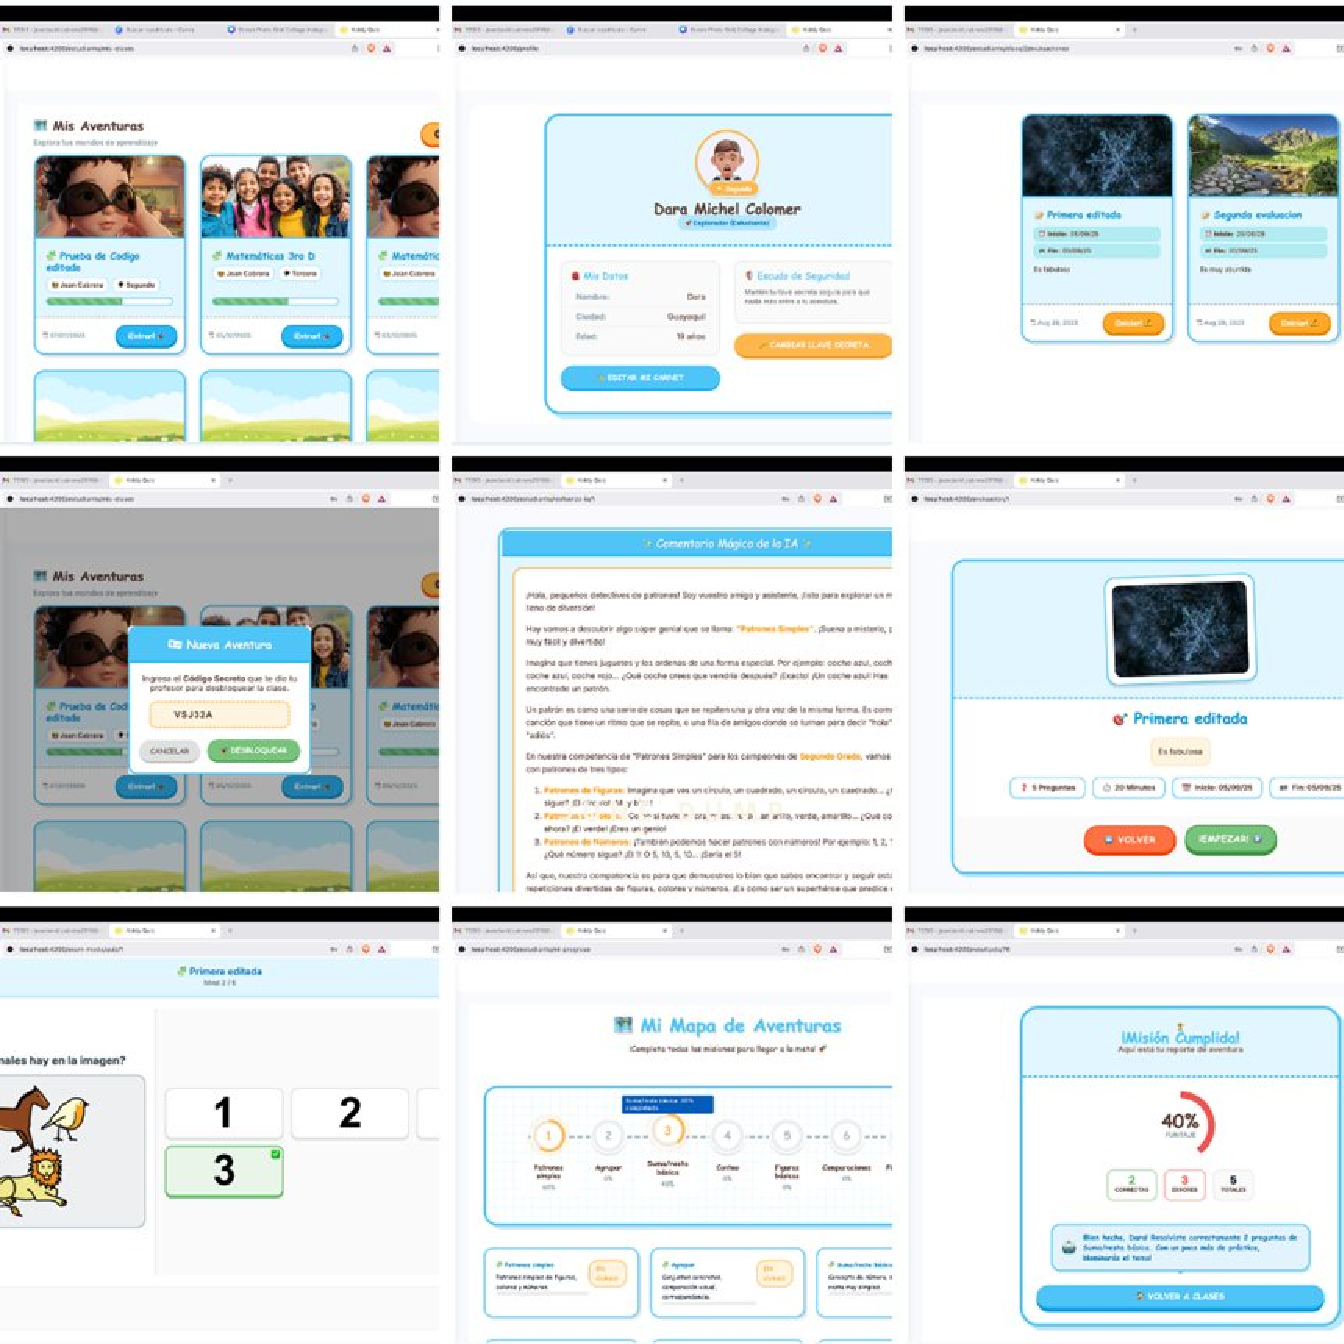
\includegraphics[width=\textwidth]{figuras/mosaico_estudiante.pdf}
\fuenteautor
\end{figure}

\begin{figure}[H]
\centering
\caption{Mosaico de pantallas implementadas para el perfil del docente.}
\label{fig:mosaico_docente}
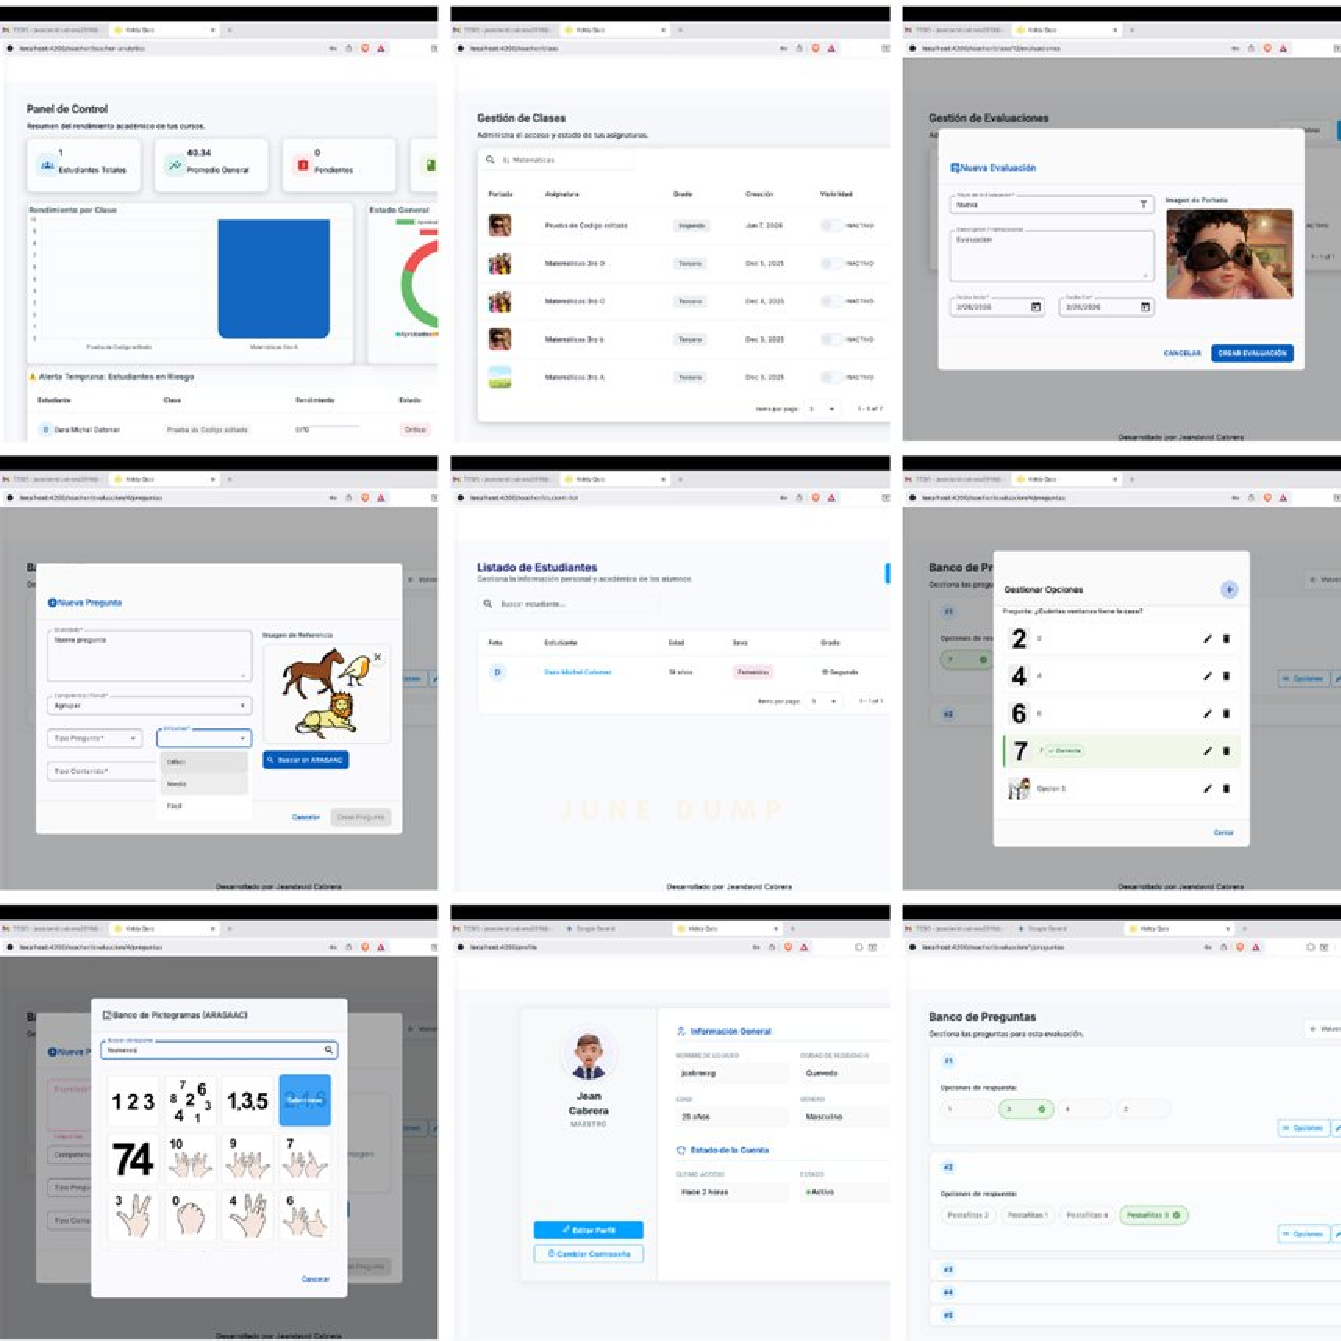
\includegraphics[width=\textwidth]{figuras/mosaico_docente.pdf}
\fuenteautor
\end{figure}

A continuación, en la Ilustración~\ref{fig:modulo_eval} se visualiza el resultado funcional y estético del módulo destinado al estudiante durante la resolución de una evaluación. La captura evidencia una navegación simplificada, adaptada a las características de la educación básica elemental, y el uso de pictogramas como apoyo visual para los enunciados matemáticos, conforme se contempla en la HU-004.1-F.

\begin{figure}[H]
\centering
\caption{Módulo del estudiante: resolución de evaluación con pictogramas.}
\label{fig:modulo_eval}
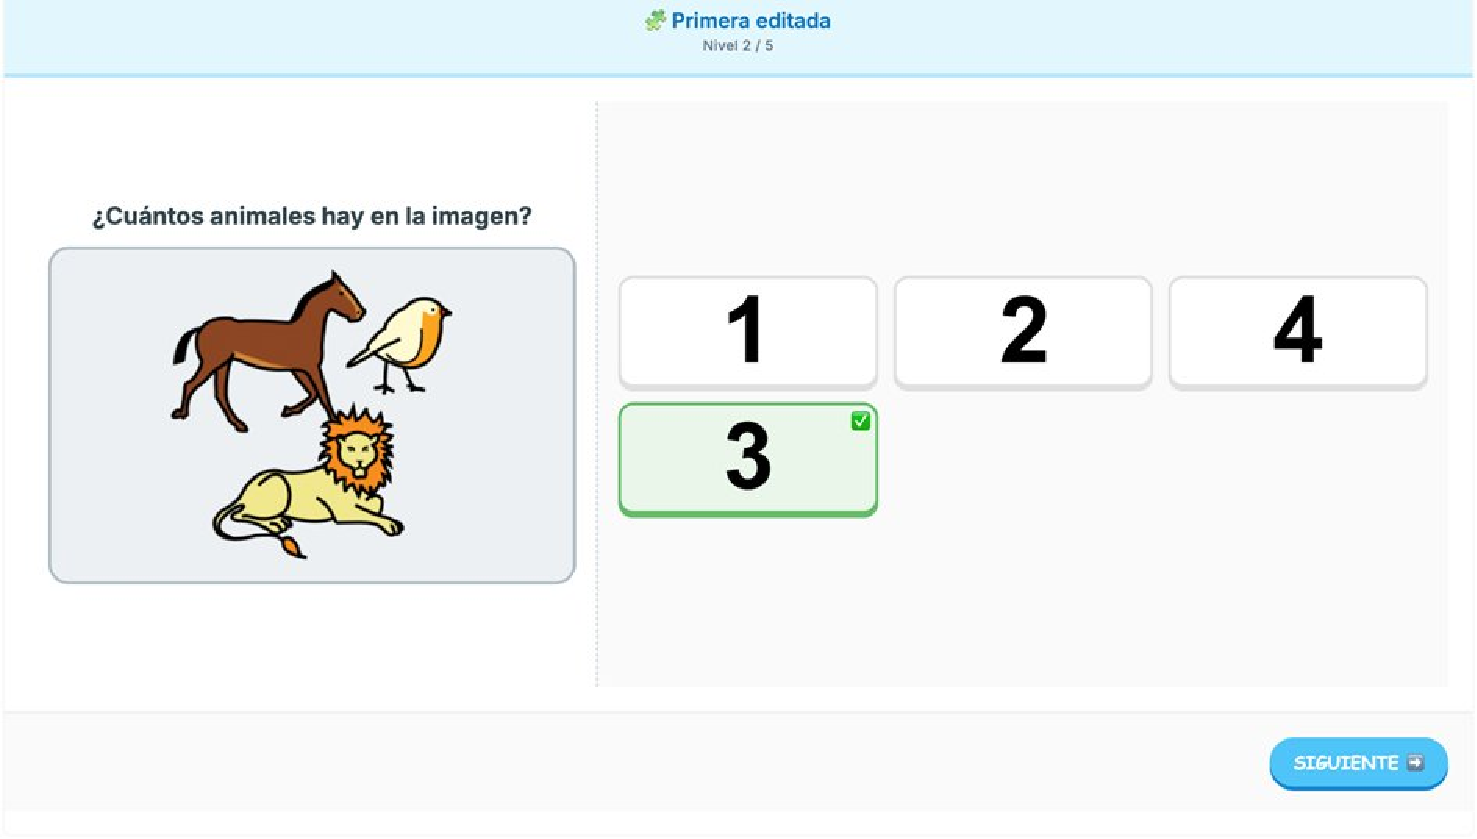
\includegraphics[width=\textwidth]{figuras/ui_resolver_eval_pictograma.pdf}
\fuenteautor
\end{figure}

La Ilustración~\ref{fig:modulo_retro} presenta la pantalla de retroalimentación motivacional posterior a la evaluación, donde se materializa la integración de Gemini AI para ofrecer un acompañamiento continuo al alumno. Se exhibe el puntaje obtenido, el desglose por aciertos y errores y un mensaje generado por la IA que invita al estudiante a continuar practicando.

\begin{figure}[H]
\centering
\caption{Módulo del estudiante: pantalla de retroalimentación con \textit{feedback} de Gemini AI.}
\label{fig:modulo_retro}
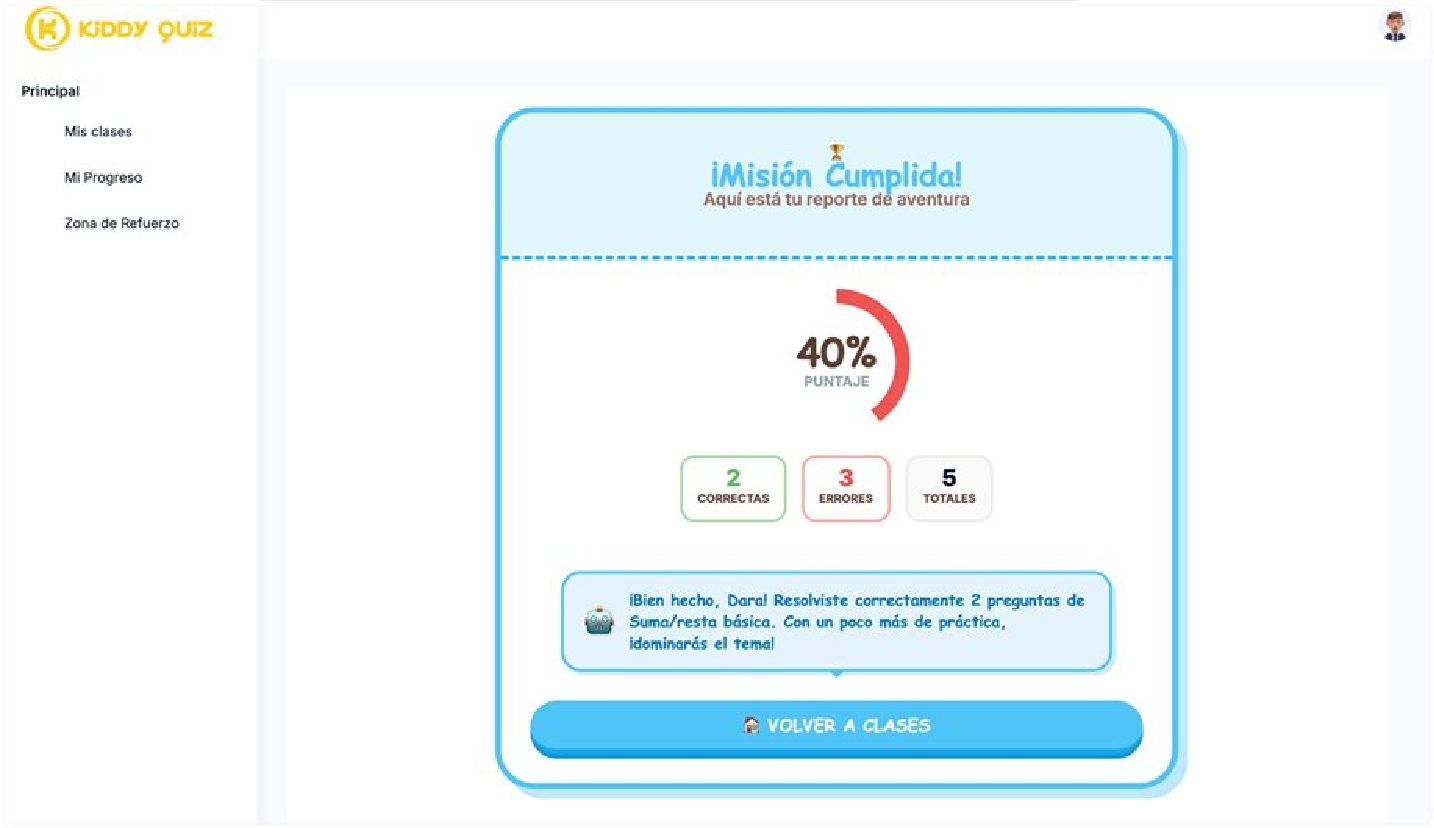
\includegraphics[width=\textwidth]{figuras/ui_retroalimentacion.pdf}
\fuenteautor
\end{figure}

En la Ilustración~\ref{fig:modulo_comentario_ia} se ilustra la sección complementaria de \textit{Comentario Mágico de la IA}, que ofrece refuerzo conceptual narrativo adaptado al lenguaje infantil para fortalecer las competencias evaluadas, atendiendo así a la HU-009.1-F y la HU-014.1-F.

\begin{figure}[H]
\centering
\caption{Sección ``Comentario Mágico de la IA'' con refuerzo narrativo de Gemini.}
\label{fig:modulo_comentario_ia}
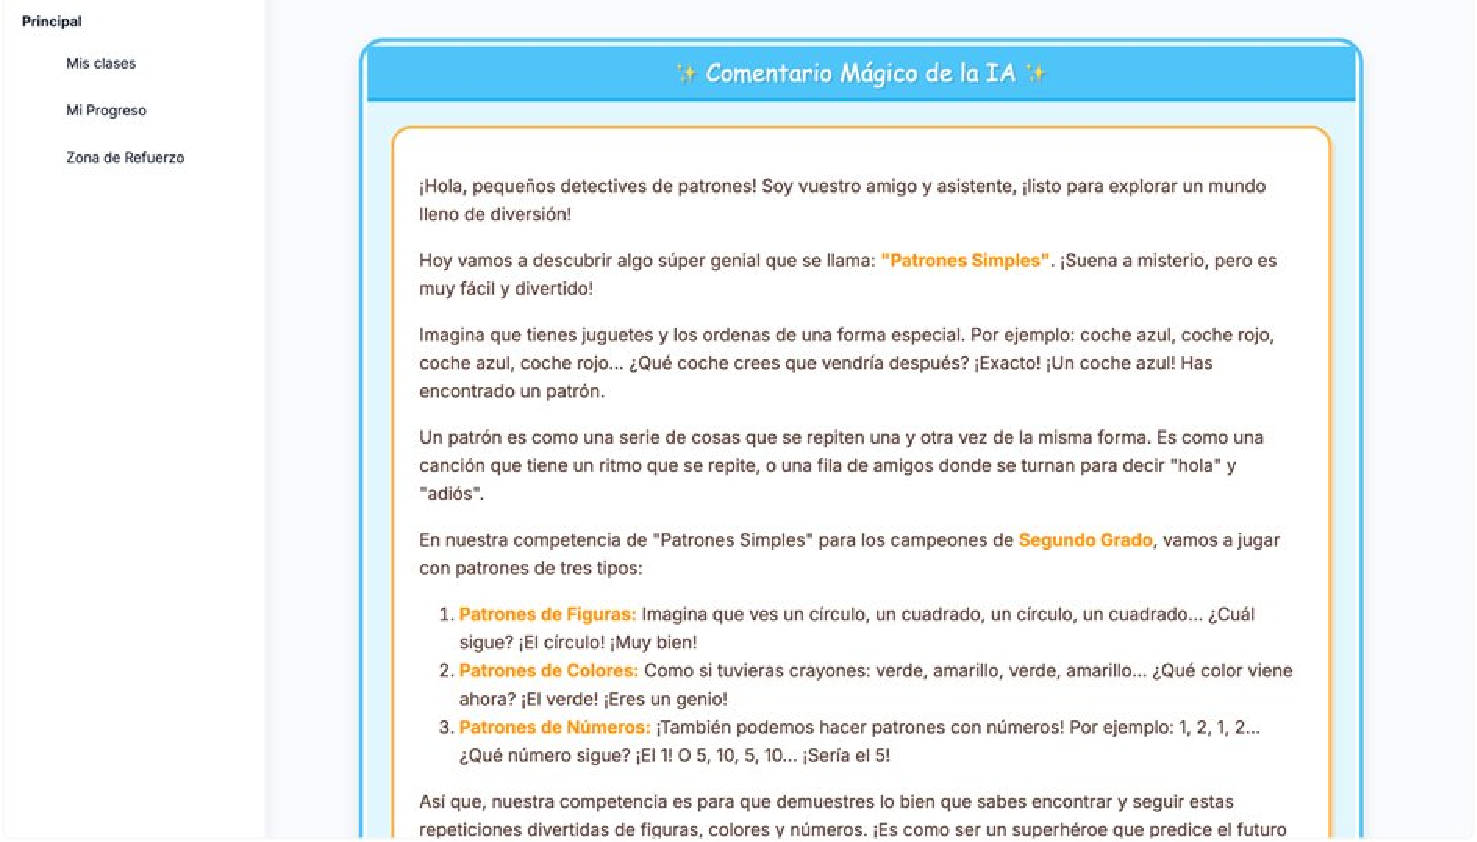
\includegraphics[width=\textwidth]{figuras/ui_comentario_magico_ia.pdf}
\fuenteautor
\end{figure}

\subsubsection*{Módulo del docente}

La Ilustración~\ref{fig:panel_docente} presenta el Panel de Control del docente, donde se centralizan los principales indicadores académicos: estudiantes totales, promedio general, evaluaciones pendientes y clases activas, junto con un acceso directo a la exportación de reportes.

\begin{figure}[H]
\centering
\caption{Panel de Control del docente con indicadores académicos consolidados.}
\label{fig:panel_docente}
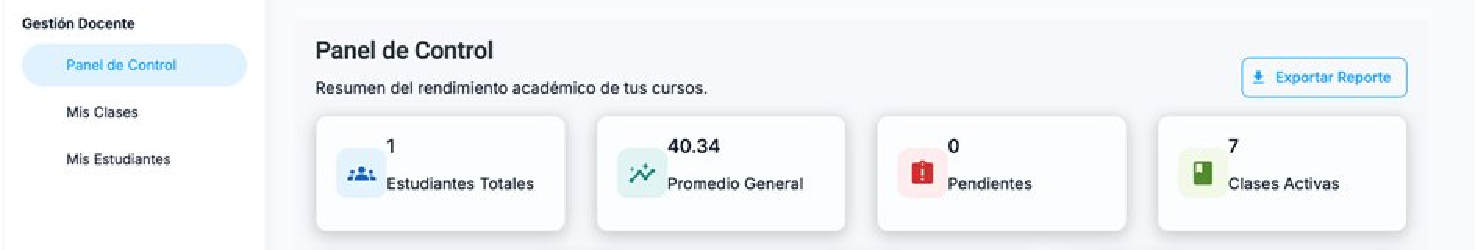
\includegraphics[width=\textwidth]{figuras/ui_panel_control_docente.pdf}
\fuenteautor
\end{figure}

La Ilustración~\ref{fig:gestion_clases} muestra la pantalla de Gestión de Clases del docente, donde se presenta la lista de cursos creados con sus respectivos atributos (portada, asignatura, grado, fecha de creación y visibilidad activa o inactiva), permitiendo al profesor controlar de manera ágil el estado de cada curso, conforme a la HU-006.1-F y la HU-006.2-F.

\begin{figure}[H]
\centering
\caption{Pantalla de Gestión de Clases del docente.}
\label{fig:gestion_clases}
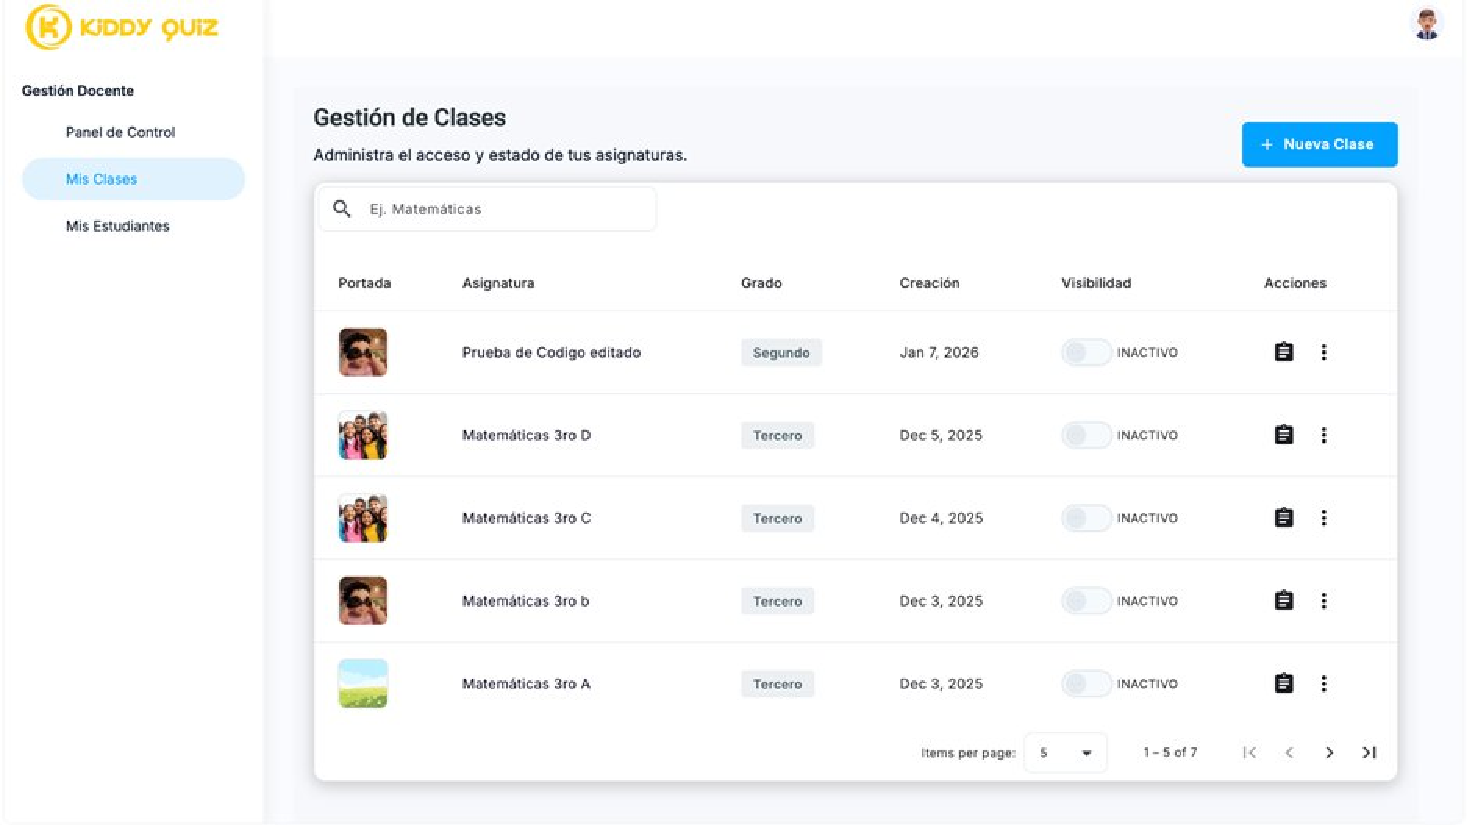
\includegraphics[width=\textwidth]{figuras/ui_panel_docente_clases.pdf}
\fuenteautor
\end{figure}

La Ilustración~\ref{fig:rendimiento_alertas} expone el panel analítico que sintetiza el Rendimiento por Clase, el Estado General de los estudiantes (aprobados, en riesgo, reprobados) y un sistema de Alerta Temprana que señala a los estudiantes con desempeño crítico, atendiendo a las HU-008.2-F, HU-008.3-F, HU-008.5-F y HU-012.1-F.

\begin{figure}[H]
\centering
\caption{Panel analítico de rendimiento con sistema de alertas tempranas.}
\label{fig:rendimiento_alertas}
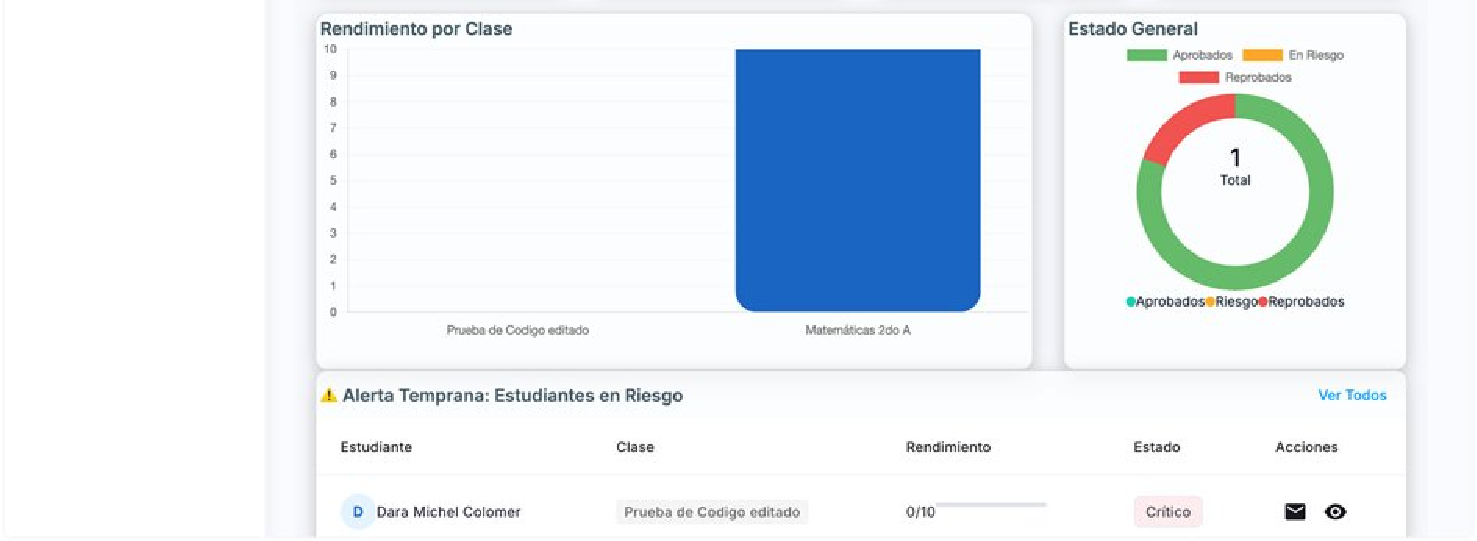
\includegraphics[width=\textwidth]{figuras/ui_rendimiento_alertas.pdf}
\fuenteautor
\end{figure}

\subsection{Integración de Gemini AI}

La integración de la inteligencia artificial constituye uno de los ejes de mayor innovación tecnológica dentro del proyecto Kiddy Quiz. Para evidenciar esta implementación, en la Ilustración~\ref{fig:gemini} se expone un fragmento del código fuente correspondiente al servicio encargado de gestionar la comunicación con dicho modelo generativo desde el \textit{backend} estructurado en NestJS.

\begin{figure}[H]
\centering
\caption{Extracto del código de integración con Gemini AI en el \textit{backend} NestJS.}
\label{fig:gemini}

\includegraphics[width=\textwidth]{figuras/fig09_gemini_ai.pdf}
\fuenteautor
\end{figure}

Para este propósito se configuró el entorno utilizando el modelo \textbf{Gemini 1.5 Flash} de Google. A diferencia de las plataformas que ofrecen calificaciones estáticas, esta arquitectura permite procesar el desempeño del estudiante en tiempo real. Como se observa en el bloque de código, el sistema filtra los datos de la evaluación y construye un \textit{prompt} estructurado donde la inteligencia artificial asume el rol de un asistente académico. Las instrucciones programadas exigen que el modelo devuelva un reporte exhaustivo en formato Markdown, el cual incluye obligatoriamente: información general de la participación, resultados detallados por pregunta, análisis de fortalezas, identificación de áreas de oportunidad y recomendaciones académicas. Esta configuración asegura que el estudiante no solo reciba una nota, sino una retroalimentación formativa, automatizada y contextualizada, fundamental para el fortalecimiento de las competencias matemáticas.

\subsection{Seguridad y autenticación}

Para garantizar la integridad de la información y la privacidad de los usuarios, la plataforma implementa un modelo de seguridad basado en JSON Web Tokens (JWT), gestionado centralmente desde el \textit{backend} con el \textit{framework} NestJS. En la Ilustración~\ref{fig:jwt} se detalla el flujo de autenticación adoptado por el sistema. El proceso inicia cuando el usuario ingresa sus credenciales, las cuales son validadas comprobando el \textit{hash} de la contraseña contra la base de datos PostgreSQL. Tras una validación exitosa, el servidor emite un token JWT firmado criptográficamente, el cual es almacenado en el cliente y utilizado en el encabezado de autorización (esquema \textit{Bearer}) en las peticiones subsecuentes.

\begin{figure}[H]
\centering
\caption{Flujo de autenticación por JWT en Kiddy Quiz.}
\label{fig:jwt}

\includegraphics[width=\textwidth]{figuras/fig10_jwt.pdf}
\fuenteautor
\end{figure}

Este mecanismo de tokens no solo protege las sesiones, sino que fundamenta el control de acceso basado en roles (RBAC) del sistema. Al interceptar la petición y extraer el \textit{payload} con métodos de verificación, el \textit{backend} identifica de manera inmediata si la petición proviene de un perfil de estudiante o de un docente, restringiendo los permisos en las rutas de la API. En caso de detectar un token inválido o permisos insuficientes, el sistema deniega el acceso retornando los códigos de estado HTTP correspondientes (401 No autorizado o 403 Acceso prohibido).

\section{Comprobación}

En esta sección se presenta la validación integral del proyecto tecnológico desarrollado, evidenciando su correcto funcionamiento y evaluando su desempeño en función de los indicadores de evaluación previamente establecidos en la sección~3.5. Estos parámetros fueron definidos para asegurar que Kiddy Quiz cumpla con los requerimientos pedagógicos y técnicos iniciales, permitiendo medir de forma objetiva su calidad, su rendimiento técnico y su nivel de aceptación por parte de los usuarios.

\subsection{Cumplimiento de plazos}

En la Ilustración~\ref{fig:plazos} se expone una comparativa detallada entre las fechas establecidas inicialmente en la planificación del proyecto y las fechas efectivas en las que se dio cumplimiento a cada uno de los hitos. Cabe destacar que, debido a la naturaleza iterativa de la metodología ágil de Programación Extrema, el cronograma mantuvo un enfoque flexible. En consecuencia, las fechas de finalización de ciertos módulos experimentaron ligeros ajustes con el propósito de incorporar correcciones, mejoras de usabilidad y refactorizaciones de código, garantizando así la calidad del producto final dentro de las treinta y dos semanas estipuladas.

\begin{figure}[H]
\centering
\caption{Cumplimiento de plazos por fase del proyecto Kiddy Quiz.}
\label{fig:plazos}

\includegraphics[width=0.95\textwidth]{figuras/fig11_cumplimiento_plazos.pdf}
\fuenteautor
\end{figure}

El cumplimiento promedio global se situó en 96,6\,\%, superando holgadamente el criterio mínimo de 90\,\% establecido en la Tabla~\ref{tab:ind_plazos}.

\subsection{Nivel de aceptación de usuario}

El análisis del nivel de usabilidad y aceptación tecnológica de la plataforma Kiddy Quiz se llevó a cabo mediante la aplicación de la Escala de Usabilidad del Sistema (SUS) y el Modelo de Aceptación Tecnológica (TAM). Estos instrumentos permitieron evaluar de forma objetiva la facilidad de interacción, la utilidad pedagógica percibida y la experiencia general tanto de los estudiantes como de los docentes al utilizar la aplicación. Los resultados consolidados de ambas pruebas demuestran que el sistema no solo cumple satisfactoriamente con las expectativas de los usuarios, sino que facilita un entorno educativo altamente funcional e intuitivo.

\subsubsection{Resultados de las evaluaciones de usabilidad (SUS)}

Para evaluar de manera exhaustiva la usabilidad de la plataforma se aplicó la Escala de Usabilidad del Sistema (SUS). El análisis descriptivo de los datos recopilados, segmentado por los dos grupos principales de usuarios (docentes y estudiantes), demuestra un nivel de accesibilidad y diseño excepcional. Como se detalla en la Tabla~\ref{tab:sus}, las métricas de tendencia central reflejan un desempeño sobresaliente. El grupo de estudiantes otorgó una calificación promedio de 87,7 sobre 100, con una mediana de 87,5, lo que evidencia una interacción sumamente fluida e intuitiva. Por su parte, el grupo de docentes registró una media favorable de 81,0 y una mediana de 82,5.

\begin{table}[H]
\centering
\caption{Resultados del cuestionario SUS aplicado a Kiddy Quiz.}
\label{tab:sus}
\begin{tabularx}{\textwidth}{|L{4.5cm}|C{3cm}|C{3cm}|}
\hline
\rowcolor{tabhead}
\tabhead{Métrica estadística} & \tabhead{Estudiantes (N=15)} & \tabhead{Docentes (N=5)}\\
\hline
Media & 87,7 & 81,0\\
\hline
Mediana & 87,5 & 82,5\\
\hline
Desviación estándar & 7,8 & 9,4\\
\hline
Valor mínimo & 80,0 & 67,5\\
\hline
Valor máximo & 95,0 & 95,0\\
\hline
\end{tabularx}
\fuenteautor
\end{table}

Resulta fundamental destacar el valor mínimo obtenido en la muestra de estudiantes, el cual se situó en 80,0. Este dato estadístico es de vital importancia, ya que confirma que ningún niño experimentó dificultades severas al navegar por los módulos o al momento de resolver sus evaluaciones. Asimismo, las desviaciones estándar (7,8 para estudiantes y 9,4 para docentes) sugieren un consenso generalizado sobre la calidad de la experiencia de usuario, superando holgadamente el puntaje de 68,0 considerado como el estándar mínimo aceptable en la industria.

Con el propósito de ilustrar el posicionamiento de estos resultados frente a los estándares internacionales de usabilidad, la Ilustración~\ref{fig:sus} despliega un gráfico de barras que contrasta las puntuaciones medias obtenidas. En esta representación visual se aprecia claramente cómo ambos perfiles de usuario superan la línea base de los 68 puntos, ubicándose firmemente dentro de la zona de aceptabilidad y excelencia.

\begin{figure}[H]
\centering
\caption{Resultados del cuestionario SUS – Aplicación Kiddy Quiz.}
\label{fig:sus}

\includegraphics[width=0.95\textwidth]{figuras/fig12_grafico_sus.pdf}
\fuenteautor
\end{figure}

\subsubsection{Resultados del Modelo de Aceptación Tecnológica (TAM)}

Para complementar la evaluación de usabilidad se aplicó el Modelo de Aceptación Tecnológica (TAM), con el objetivo de medir empíricamente la viabilidad pedagógica y el nivel de adopción de la plataforma. Este instrumento evalúa tres dimensiones fundamentales: la Utilidad Percibida (PU), la Facilidad de Uso Percibida (PEOU) y la Intención de Uso (IU), valoradas mediante una escala de Likert de 1 a 5.

El análisis descriptivo de las respuestas, estructurado por tipo de usuario, revela una aceptación excepcional de la herramienta, destacando una tendencia sumamente positiva por parte del grupo de estudiantes. Al observar los estadísticos de tendencia central se evidencia que los niños perciben una mayor facilidad al navegar por la plataforma (media de 4,78) en comparación con los docentes (media de 3,95). Este contraste valida contundentemente la eficacia del diseño de interfaz centrado en el usuario infantil: el uso de pictogramas y elementos visuales simplificados logró que los estudiantes interactuaran con el sistema de forma más natural e intuitiva que los propios adultos. Asimismo, la baja desviación estándar en las métricas de los estudiantes (oscilando entre 0,14 y 0,23) indica un alto grado de consenso, confirmando que la experiencia positiva fue generalizada y no un caso aislado.

El hallazgo más significativo dentro de esta evaluación recae en la dimensión de Intención de Uso. El grupo de estudiantes registró una media de 4,93 y una mediana perfecta de 5,0, con un valor mínimo de 4,6. Esta calificación, que roza el límite superior absoluto de la escala, demuestra un nivel de motivación intrínseca sobresaliente, atribuible directamente a la innovación central del proyecto: la integración de retroalimentación generada por Inteligencia Artificial.

\begin{table}[H]
\centering
\caption{Resultados del cuestionario TAM aplicado a Kiddy Quiz.}
\label{tab:tam}
\begin{small}
\begin{tabularx}{\textwidth}{|L{3.7cm}|L{2.7cm}|C{1.4cm}|C{1.6cm}|X|}
\hline
\rowcolor{tabhead}
\tabhead{Dimensión} & \tabhead{Grupo} & \tabhead{Media} & \tabhead{Desv.~Est.} & \tabhead{Interpretación}\\
\hline
\multirow{2}{*}{Utilidad Percibida (PU)} & Docentes (N=5) & 4,45 & 0,33 & Muy alta percepción de utilidad pedagógica\\
\cline{2-5}
 & Estudiantes (N=15) & 4,85 & 0,22 & Percepción cercana al máximo absoluto\\
\hline
\multirow{2}{*}{Facilidad de Uso (PEOU)} & Docentes (N=5) & 3,95 & 0,27 & Facilidad alta, requiere mínimo esfuerzo\\
\cline{2-5}
 & Estudiantes (N=15) & 4,78 & 0,23 & Interfaz extremadamente intuitiva\\
\hline
\multirow{2}{*}{Intención de Uso (IU)} & Docentes (N=5) & 4,47 & 0,38 & Fuerte disposición a integrar la herramienta\\
\cline{2-5}
 & Estudiantes (N=15) & 4,93 & 0,14 & Intención casi unánime y máxima\\
\hline
\end{tabularx}
\end{small}
\fuenteautor
\end{table}

Para ilustrar de manera visual y comparativa los resultados estadísticos expuestos, la Ilustración~\ref{fig:tam} presenta un gráfico de brechas (\textit{Dumbbell Plot}) enfocado en las tres dimensiones del Modelo TAM. Esta representación gráfica permite contrastar de forma directa las puntuaciones medias otorgadas por docentes y estudiantes.

\begin{figure}[H]
\centering
\caption{Gráfico de brechas TAM – Comparación docentes vs.\ estudiantes.}
\label{fig:tam}
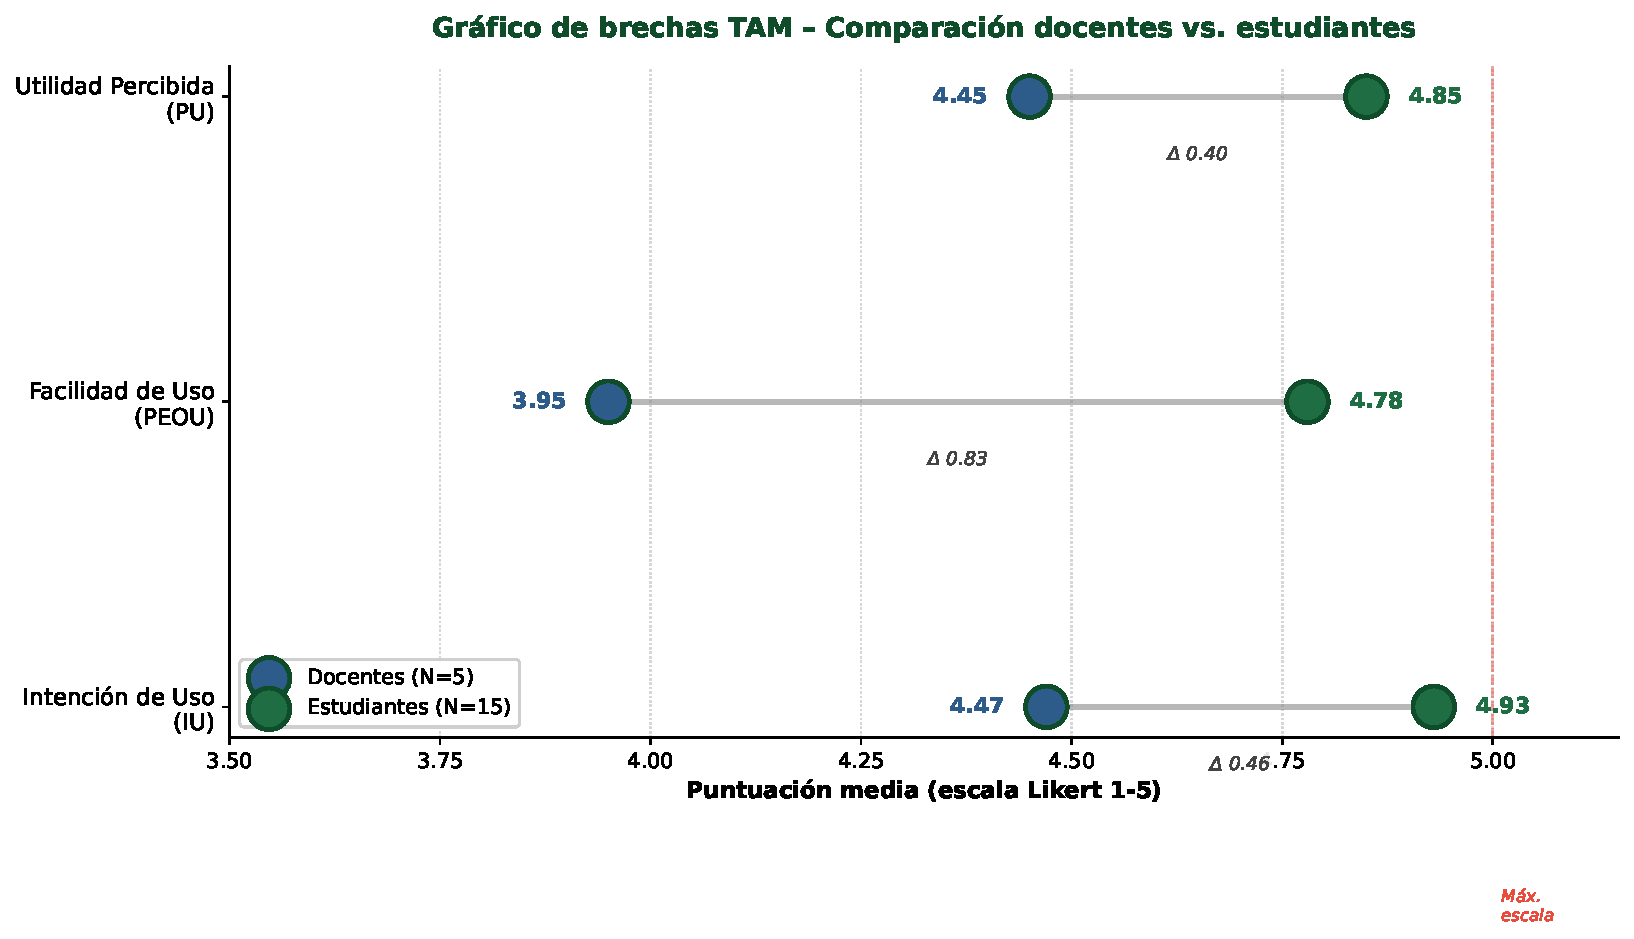
\includegraphics[width=0.95\textwidth]{figuras/fig13_grafico_tam.pdf}
\fuenteautor
\end{figure}

Como se puede observar en el gráfico, la longitud de las líneas conectoras evidencia la diferencia de percepción entre ambos perfiles de usuario. La brecha más amplia se presenta claramente en la Facilidad de Uso (PEOU), donde los estudiantes (4,78) superan de forma notoria a los docentes (3,95). Esto demuestra gráficamente que la interfaz adaptada cumplió su objetivo de reducir la carga cognitiva en los niños. Asimismo, la gráfica destaca cómo el indicador de Intención de Uso en los estudiantes alcanza el punto máximo del esquema (4,93), posicionándose casi en el límite perfecto de la escala. En conjunto, esta visualización corrobora que Kiddy Quiz logró una adopción tecnológica sobresaliente, validando el impacto positivo de la inteligencia artificial y el diseño interactivo en el público infantil.

\section{Discusión}

Los resultados obtenidos confirman la pertinencia y eficacia de la solución propuesta, en línea con la literatura existente sobre evaluación por competencias y tecnologías educativas. La puntuación SUS de 87,7 obtenida con los estudiantes ubica a Kiddy Quiz en la categoría de \textit{Excelente} según la escala de Bangor, superando los rangos típicamente reportados para herramientas similares orientadas a educación superior \cite{ref10_cat,ref21_scala_universidad}. Resulta particularmente significativa la diferencia entre la facilidad de uso percibida por los estudiantes (4,78) y la de los docentes (3,95): mientras la literatura suele reportar mayor dificultad de uso en niños debido a su menor experiencia tecnológica, en este caso el resultado se invierte gracias al diseño centrado en pictogramas y elementos visuales simplificados \cite{ref40_mayer,ref48_nielsen}, una validación empírica del principio de doble codificación \cite{ref43_paivio}.

Comparado con SCALA \cite{ref21_scala_universidad}, CAT \cite{ref10_cat} y SECAT \cite{ref11_secat}, Kiddy Quiz introduce tres diferenciadores sustantivos que constituyen su aporte original: (i) el enfoque deliberado en educación básica elemental --un nivel desatendido en la literatura existente--; (ii) la integración de retroalimentación generativa por IA, que trasciende las rúbricas estáticas de los antecedentes; y (iii) la incorporación nativa de elementos de accesibilidad visual, alineada con las recomendaciones de equidad educativa \cite{ref42_cabero}. Estos hallazgos refuerzan la tesis de que la digitalización efectiva en evaluación educativa requiere no solo plataformas funcionales, sino diseños pedagógicamente situados y empíricamente validados \cite{ref14_anderson,ref27_blackwiliam}.

Las brechas observadas entre la percepción de docentes y estudiantes coinciden con los hallazgos de Ertmer y Ottenbreit-Leftwich \cite{ref08_ertmer} sobre las barreras de adopción tecnológica del profesorado, lo que sugiere la necesidad de complementar el producto con instancias de capacitación docente. No obstante, la alta intención de uso reportada por los docentes (4,47) indica una disposición favorable hacia la incorporación de la herramienta en sus prácticas, especialmente cuando los beneficios de automatización del seguimiento académico se hacen tangibles.
